\appendix

\chapter{Supplementary Experimental Figures}
\label{app:supplementary}

This appendix reproduces archived figure sets for the four-category analysis, layer ablation, three-condition dynamical summaries, and three-condition coupling analysis. Captions use the inferential limits stated in Chapters~\ref{chap:arspi_net}--\ref{chap:synthesis}; several displayed analyses remain descriptive because raw inputs were unavailable for corrected reruns.


%% ═══════════════════════════════════════════════════════════════
%% SECTION A.1: FOUR-CLASS RAW OBSERVATIONS
%% ═══════════════════════════════════════════════════════════════
\section{Four-Class Raw Observations}
\label{app:4class_obs}

The following seven archived observation sets summarize the four affective categories before the reported classifier and clinical comparisons.

\begin{figure}[H]
    \centering
    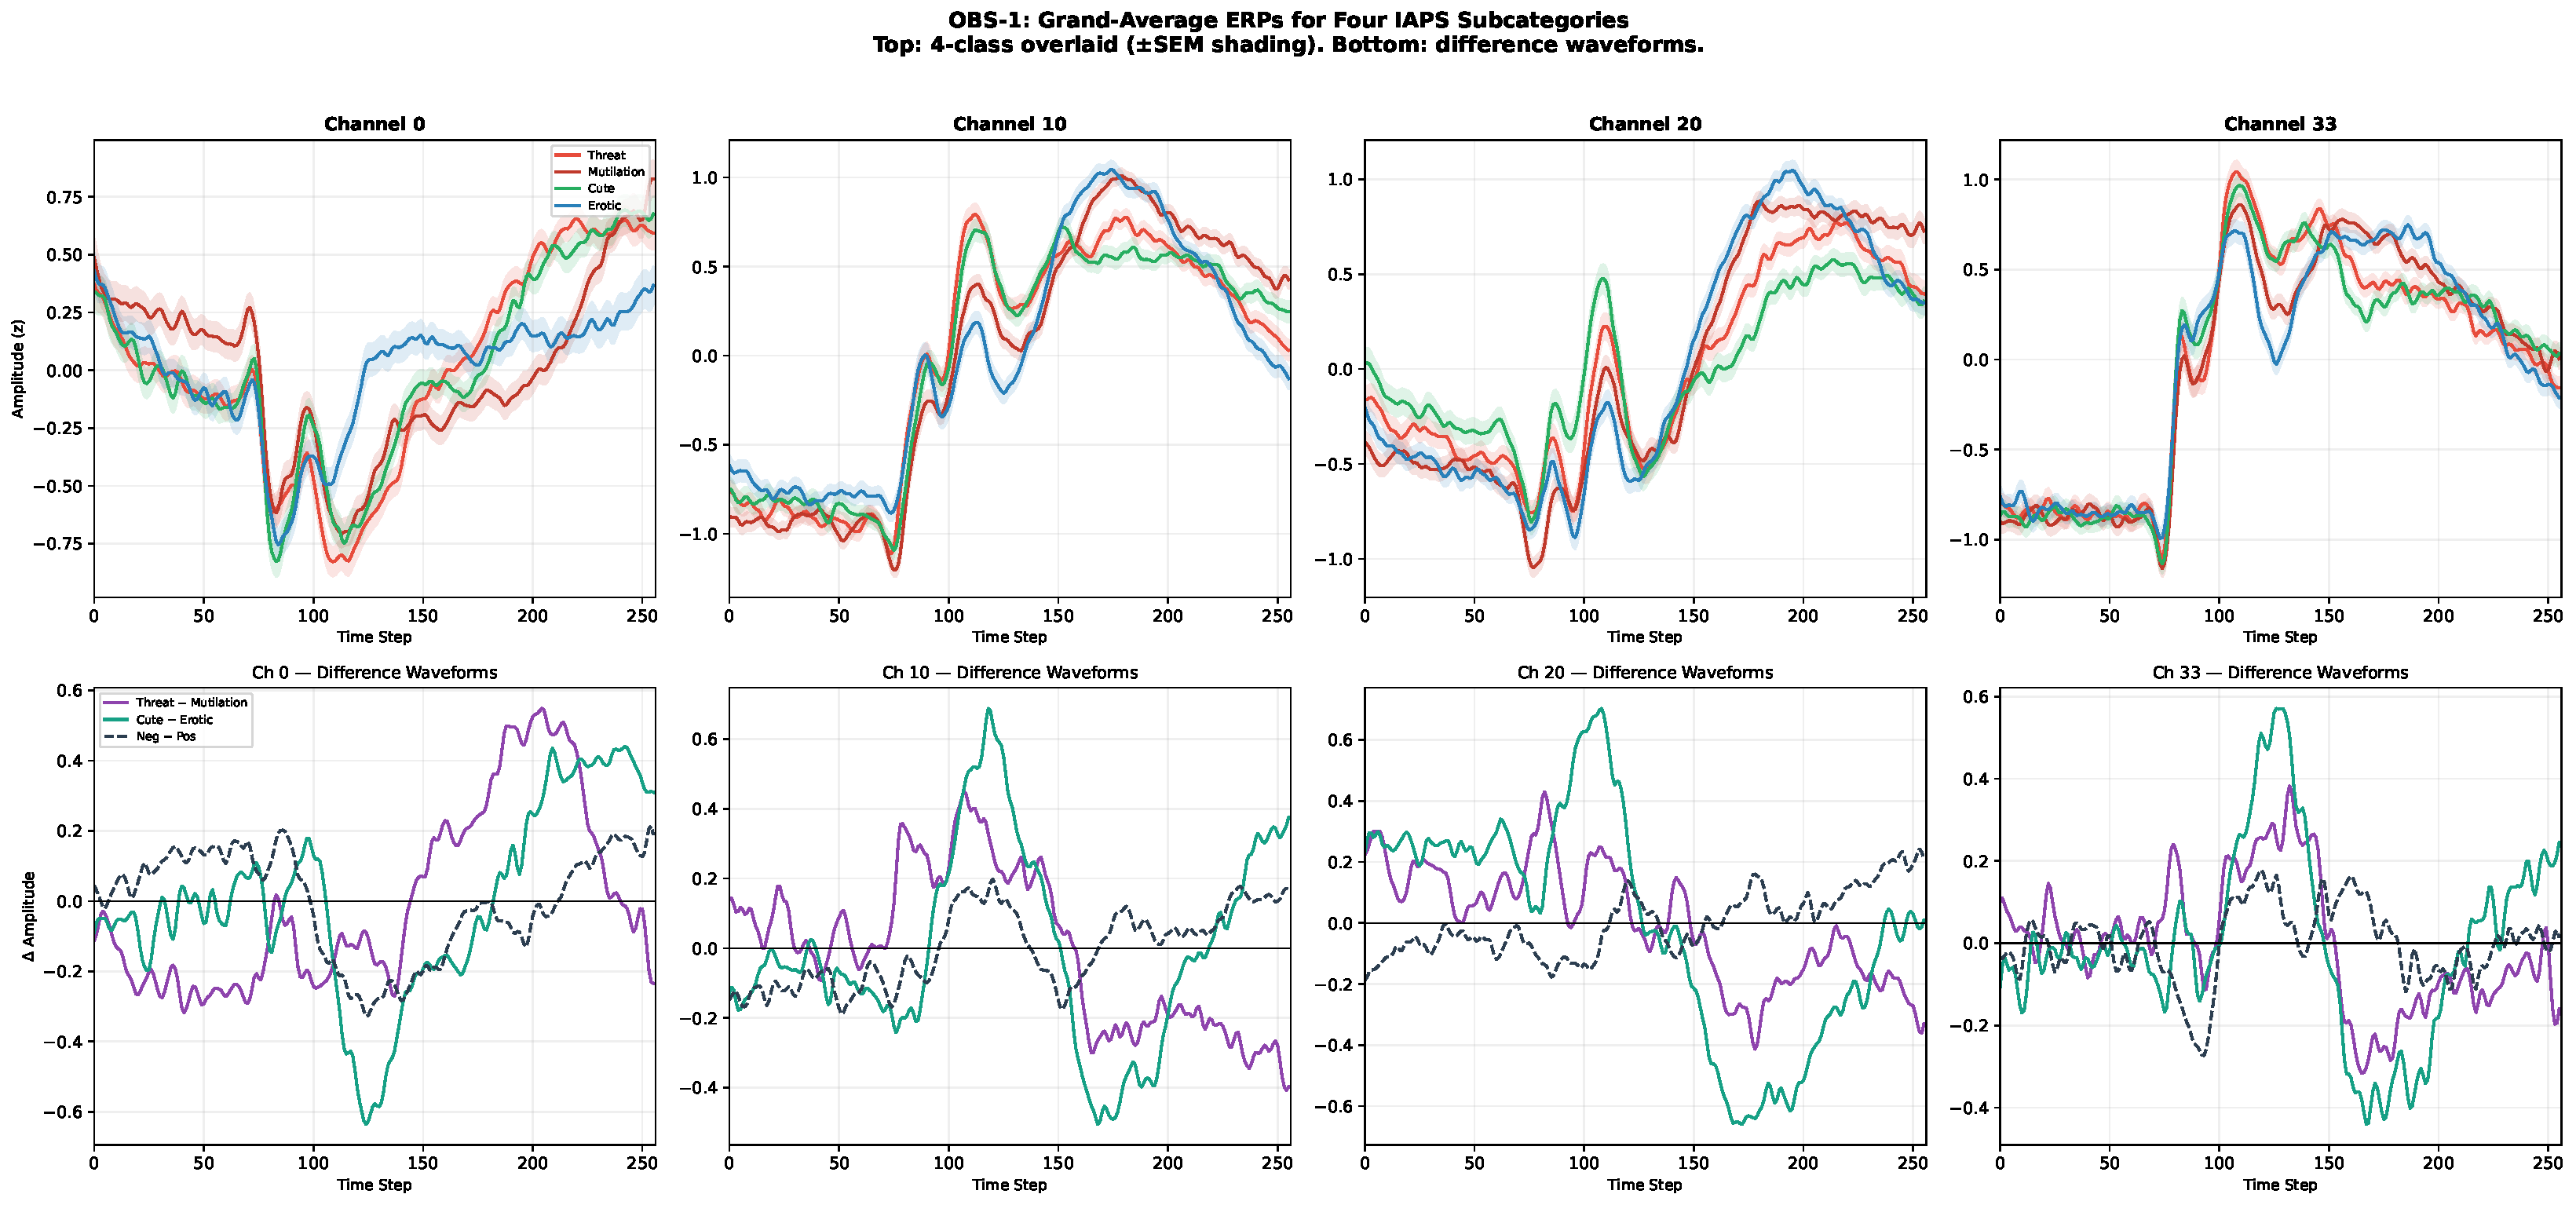
\includegraphics[width=\textwidth]{pictures/appendixA/ch5_4class_obs01_erps.pdf}
    \caption{Grand-average waveforms by category ($N=211$). The displayed late-window differences are descriptive; stimulus-level arousal and valence were not modeled separately.}
    \label{fig:app_4class_obs01}
\end{figure}

\begin{figure}[H]
    \centering
    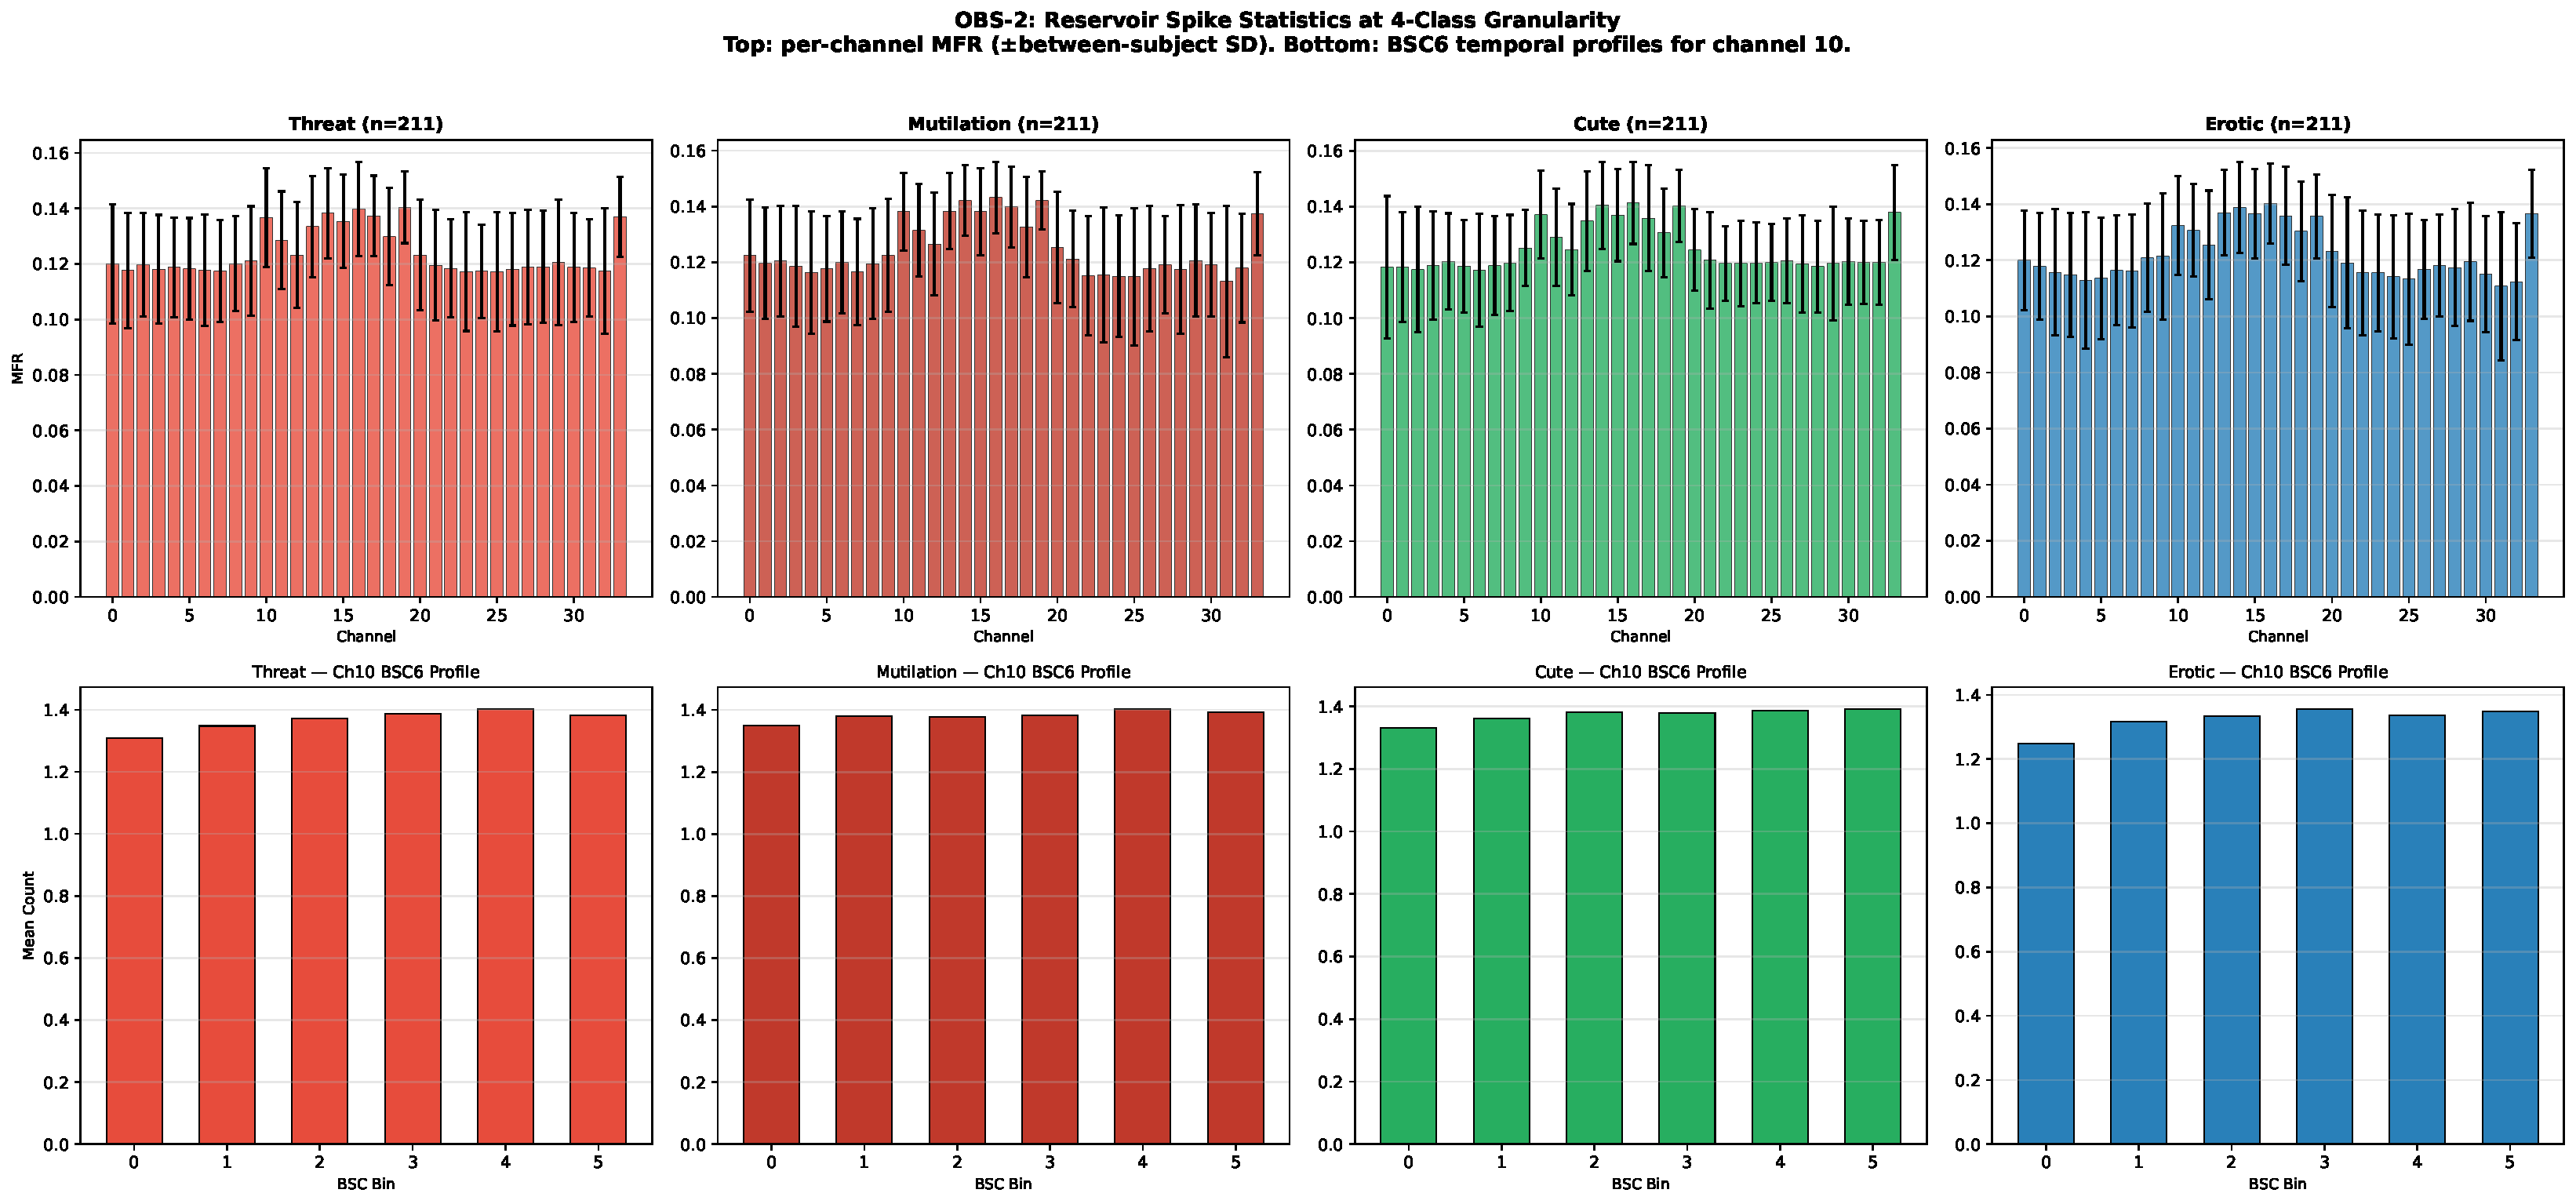
\includegraphics[width=\textwidth]{pictures/appendixA/ch5_4class_obs02_spike_stats.pdf}
    \caption{Archived reservoir spike statistics at four-category resolution: per-channel total spike counts and firing-rate distributions. Gross activation is similar across the displayed category averages; the figure is descriptive and does not test a prespecified channel family.}
    \label{fig:app_4class_obs02}
\end{figure}

\begin{figure}[H]
    \centering
    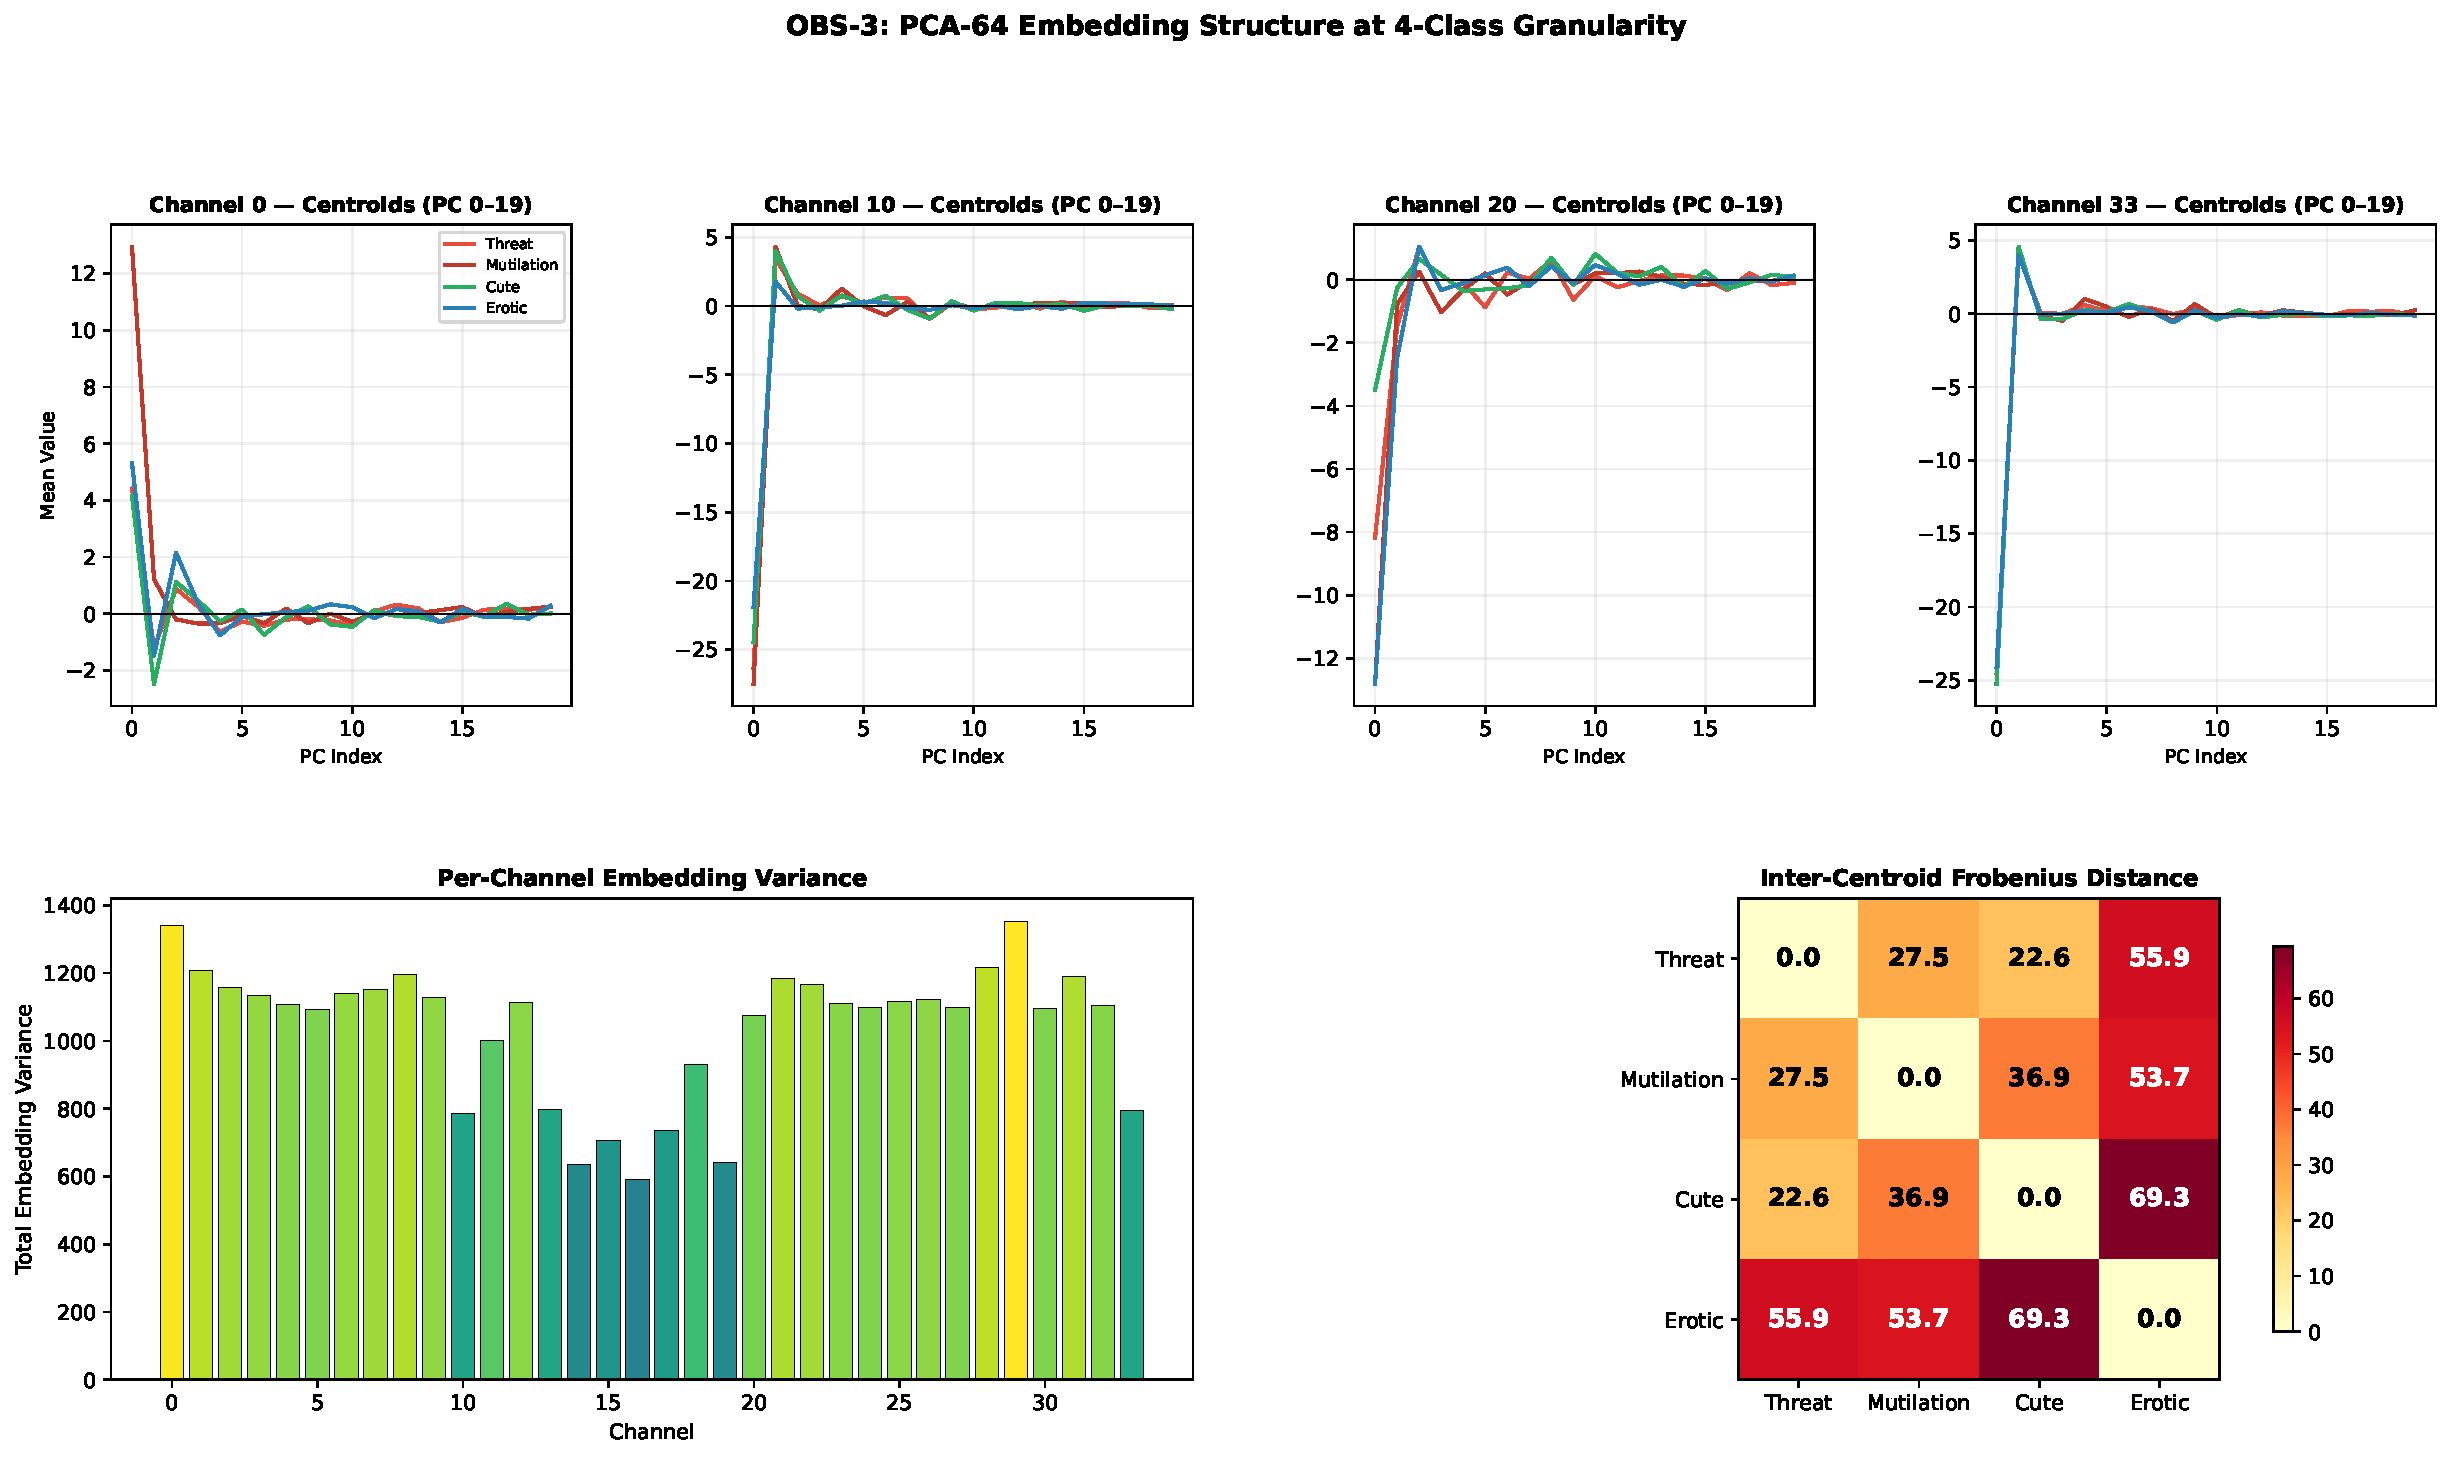
\includegraphics[width=\textwidth]{pictures/appendixA/ch5_4class_obs03_embeddings.pdf}
    \caption{Archived full-sample PCA-64 geometry at four-category resolution. A two-component projection shows substantial category overlap and visible grouping by participant. The reported sums-of-squares fractions are $2.4\%$ for category and $47.0\%$ for participant; because preprocessing and labels differ from the three-condition workflow, the two analyses are not direct replications.}
    \label{fig:app_4class_obs03}
\end{figure}

\begin{figure}[H]
    \centering
    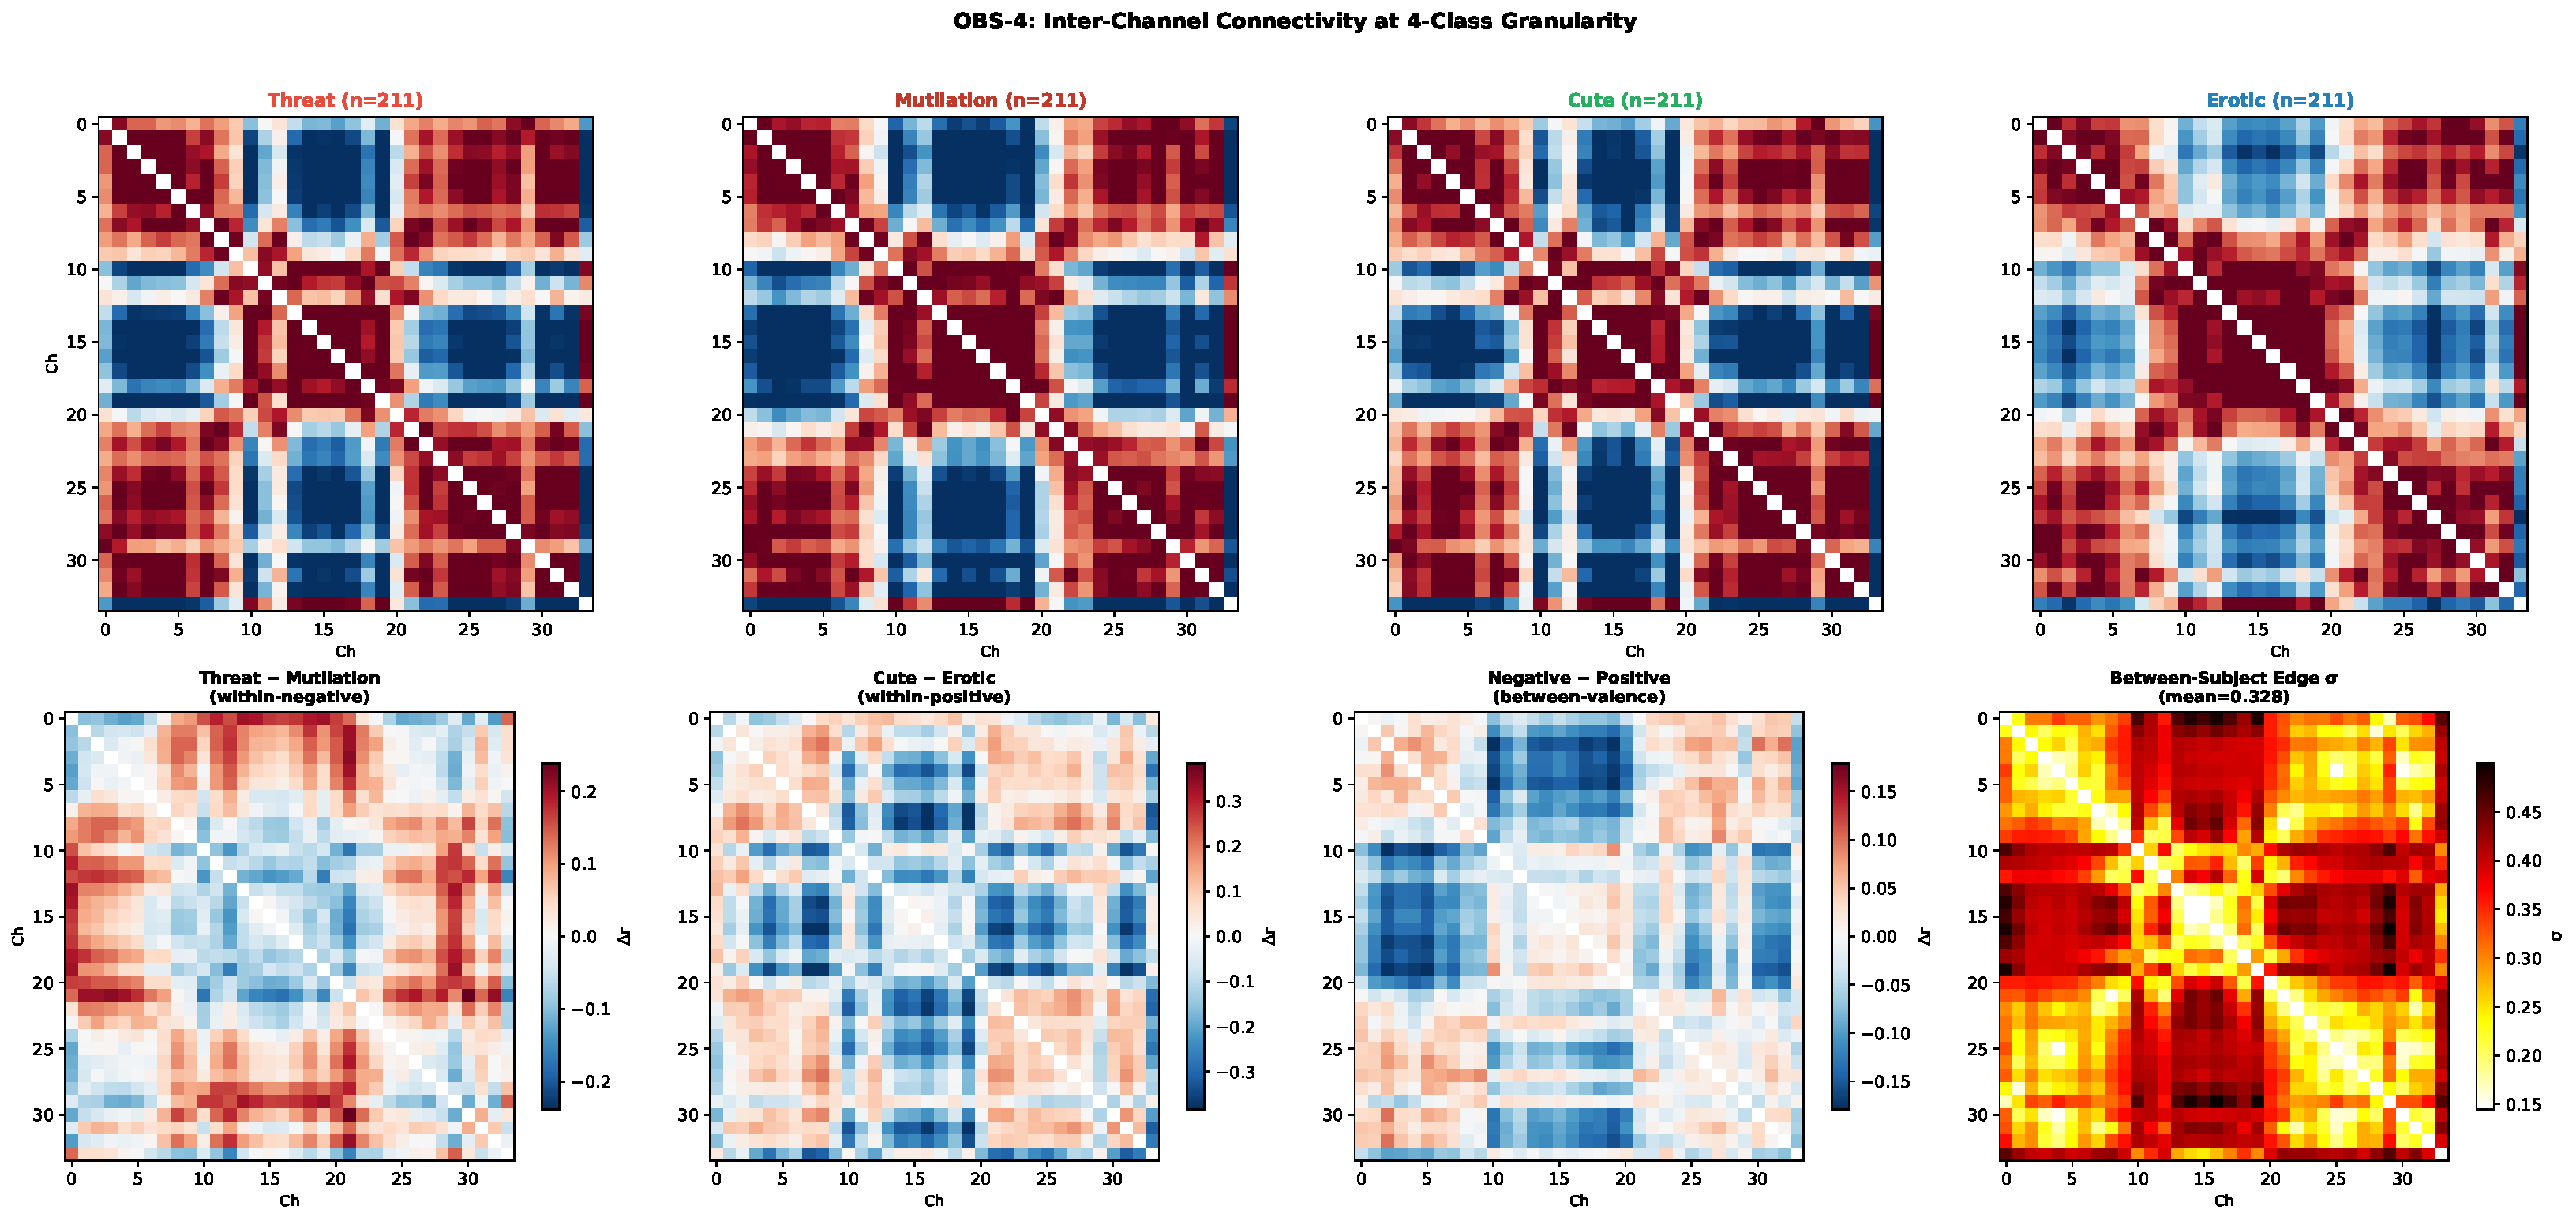
\includegraphics[width=\textwidth]{pictures/appendixA/ch5_4class_obs04_connectivity.pdf}
    \caption{Archived inter-channel representation-similarity matrices and thresholded graph summaries at four-category resolution. The matrices use unlabeled channel indices and full-sample PCA coordinates; they are not estimates of physiological connectivity or anatomical networks.}
    \label{fig:app_4class_obs04}
\end{figure}

\begin{figure}[H]
    \centering
    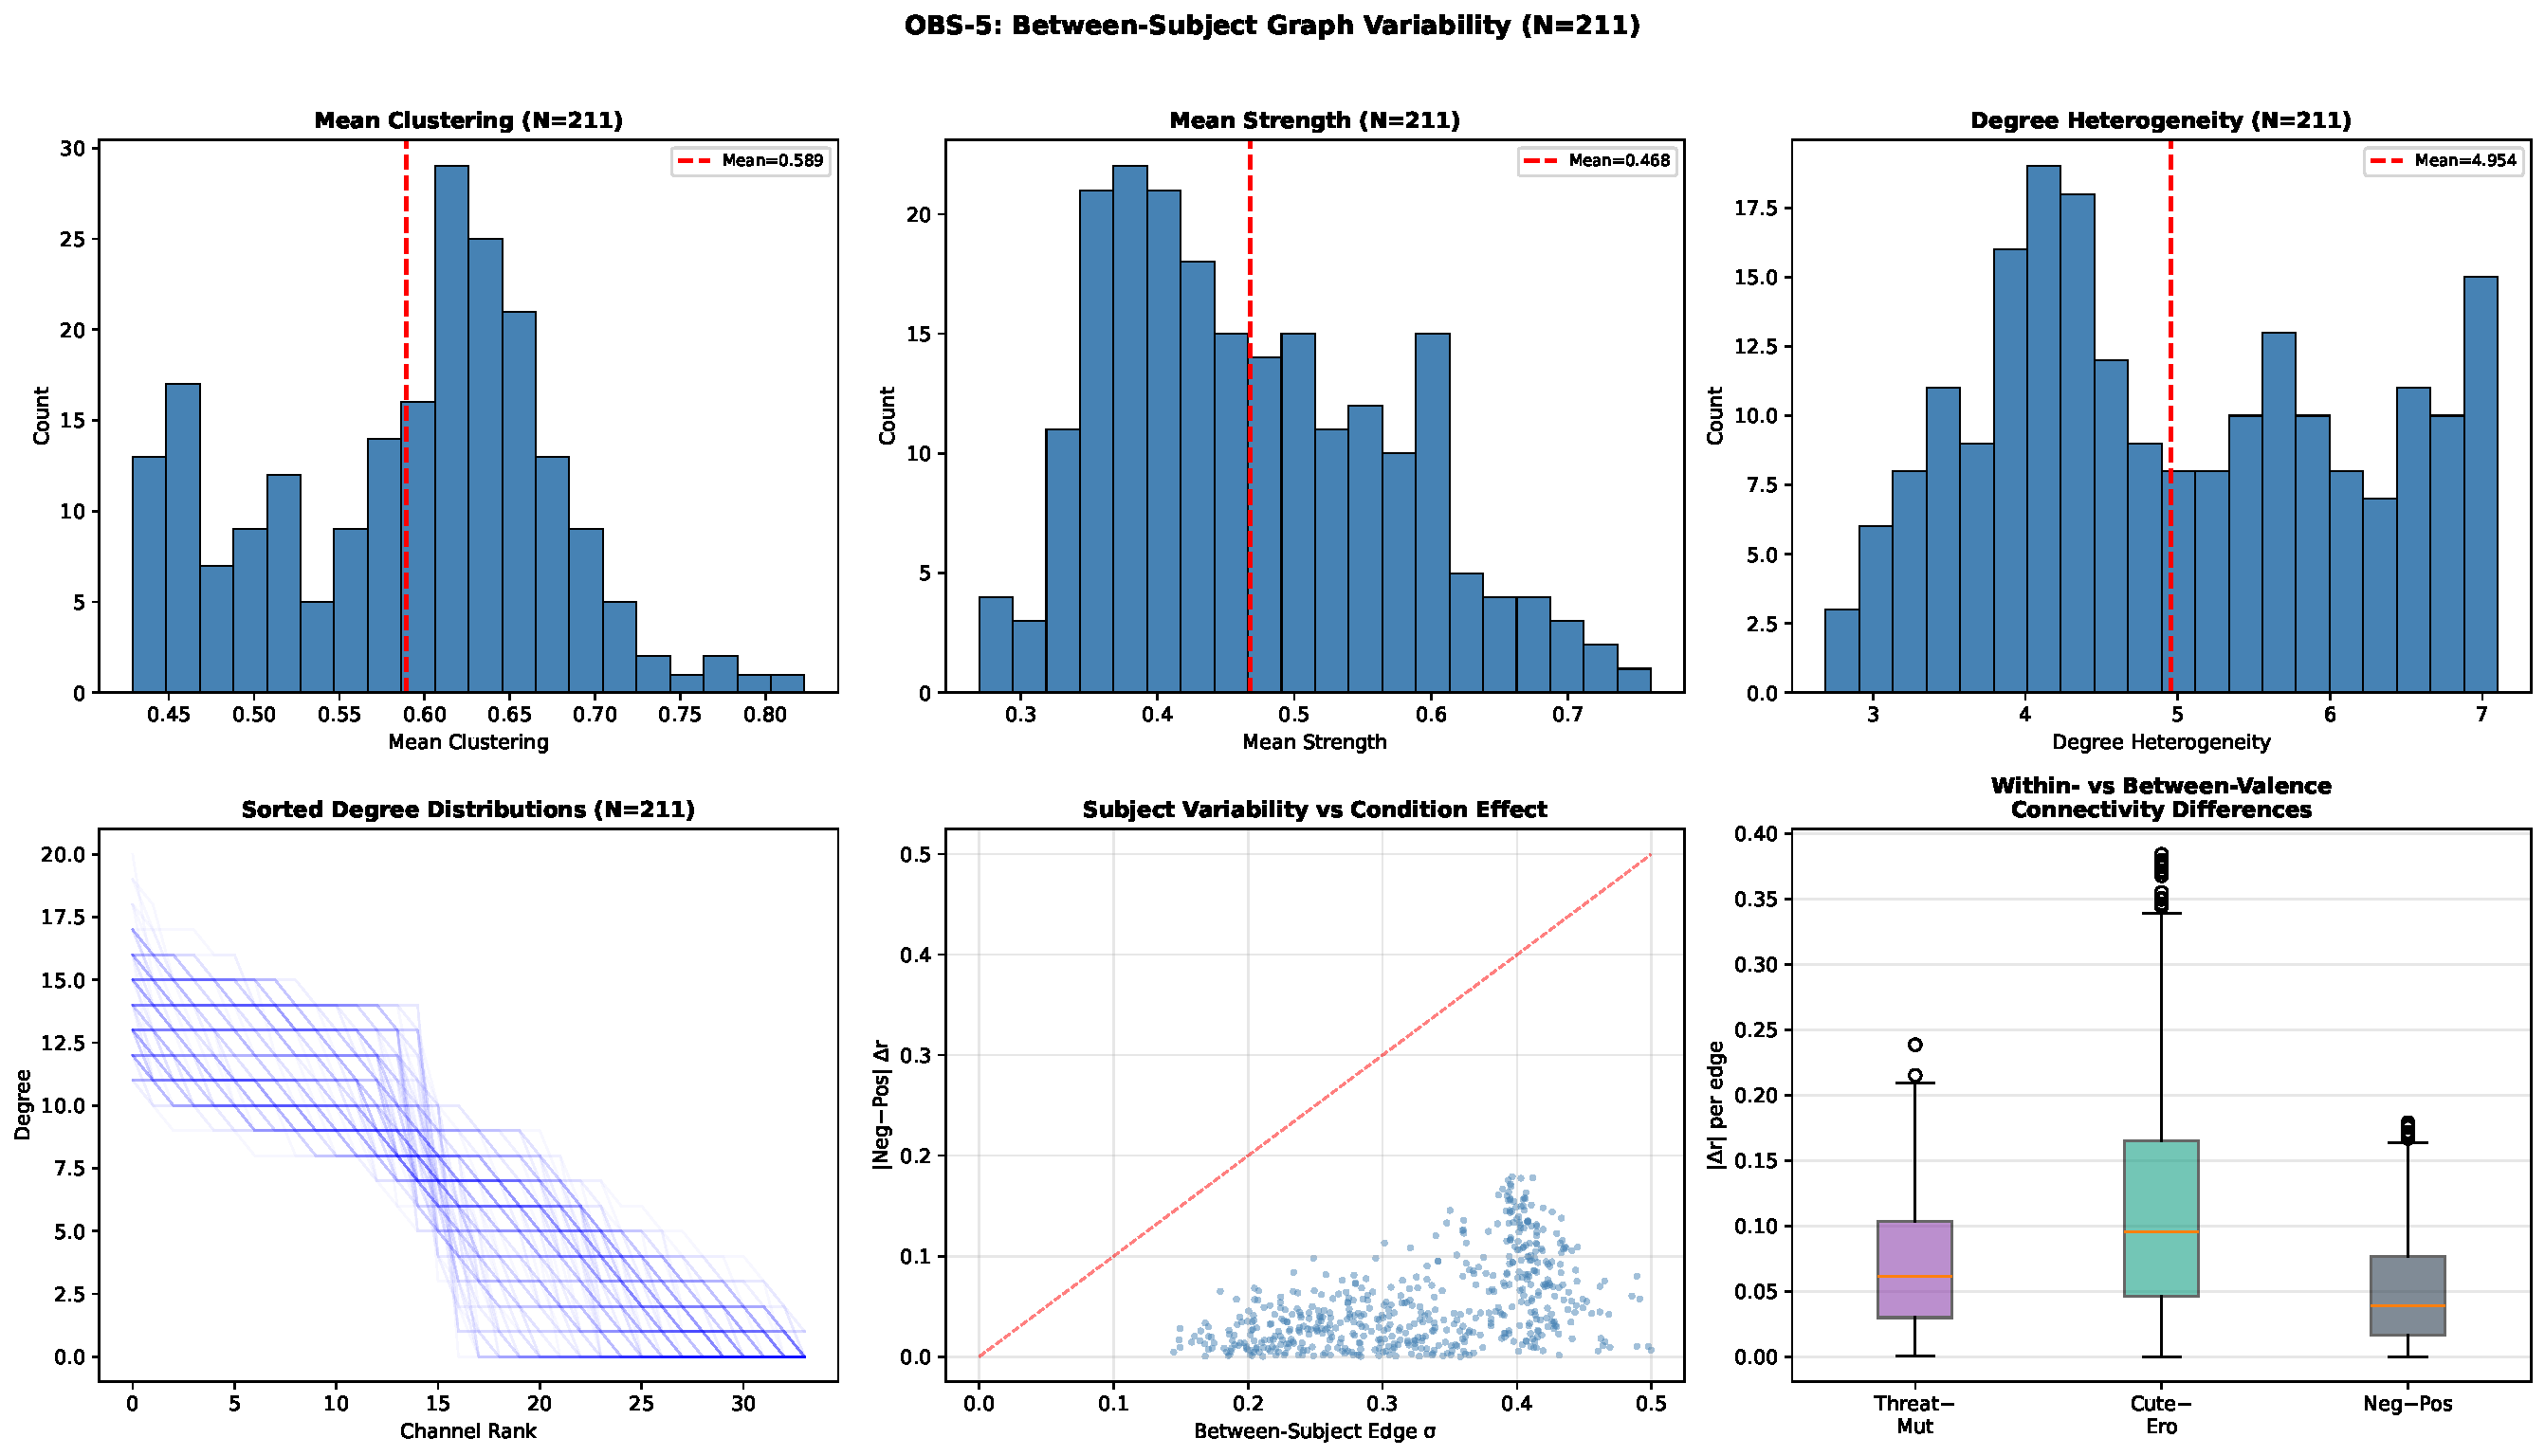
\includegraphics[width=\textwidth]{pictures/appendixA/ch5_4class_obs05_graph_variability.pdf}
    \caption{Archived between-participant graph variability at four-category resolution. The reported participant-to-category sums-of-squares ratio is $19.6\times$, compared with $7.2\times$ in the unmatched three-condition workflow. The ratio is descriptive and does not establish trait stability.}
    \label{fig:app_4class_obs05}
\end{figure}

\begin{figure}[H]
    \centering
    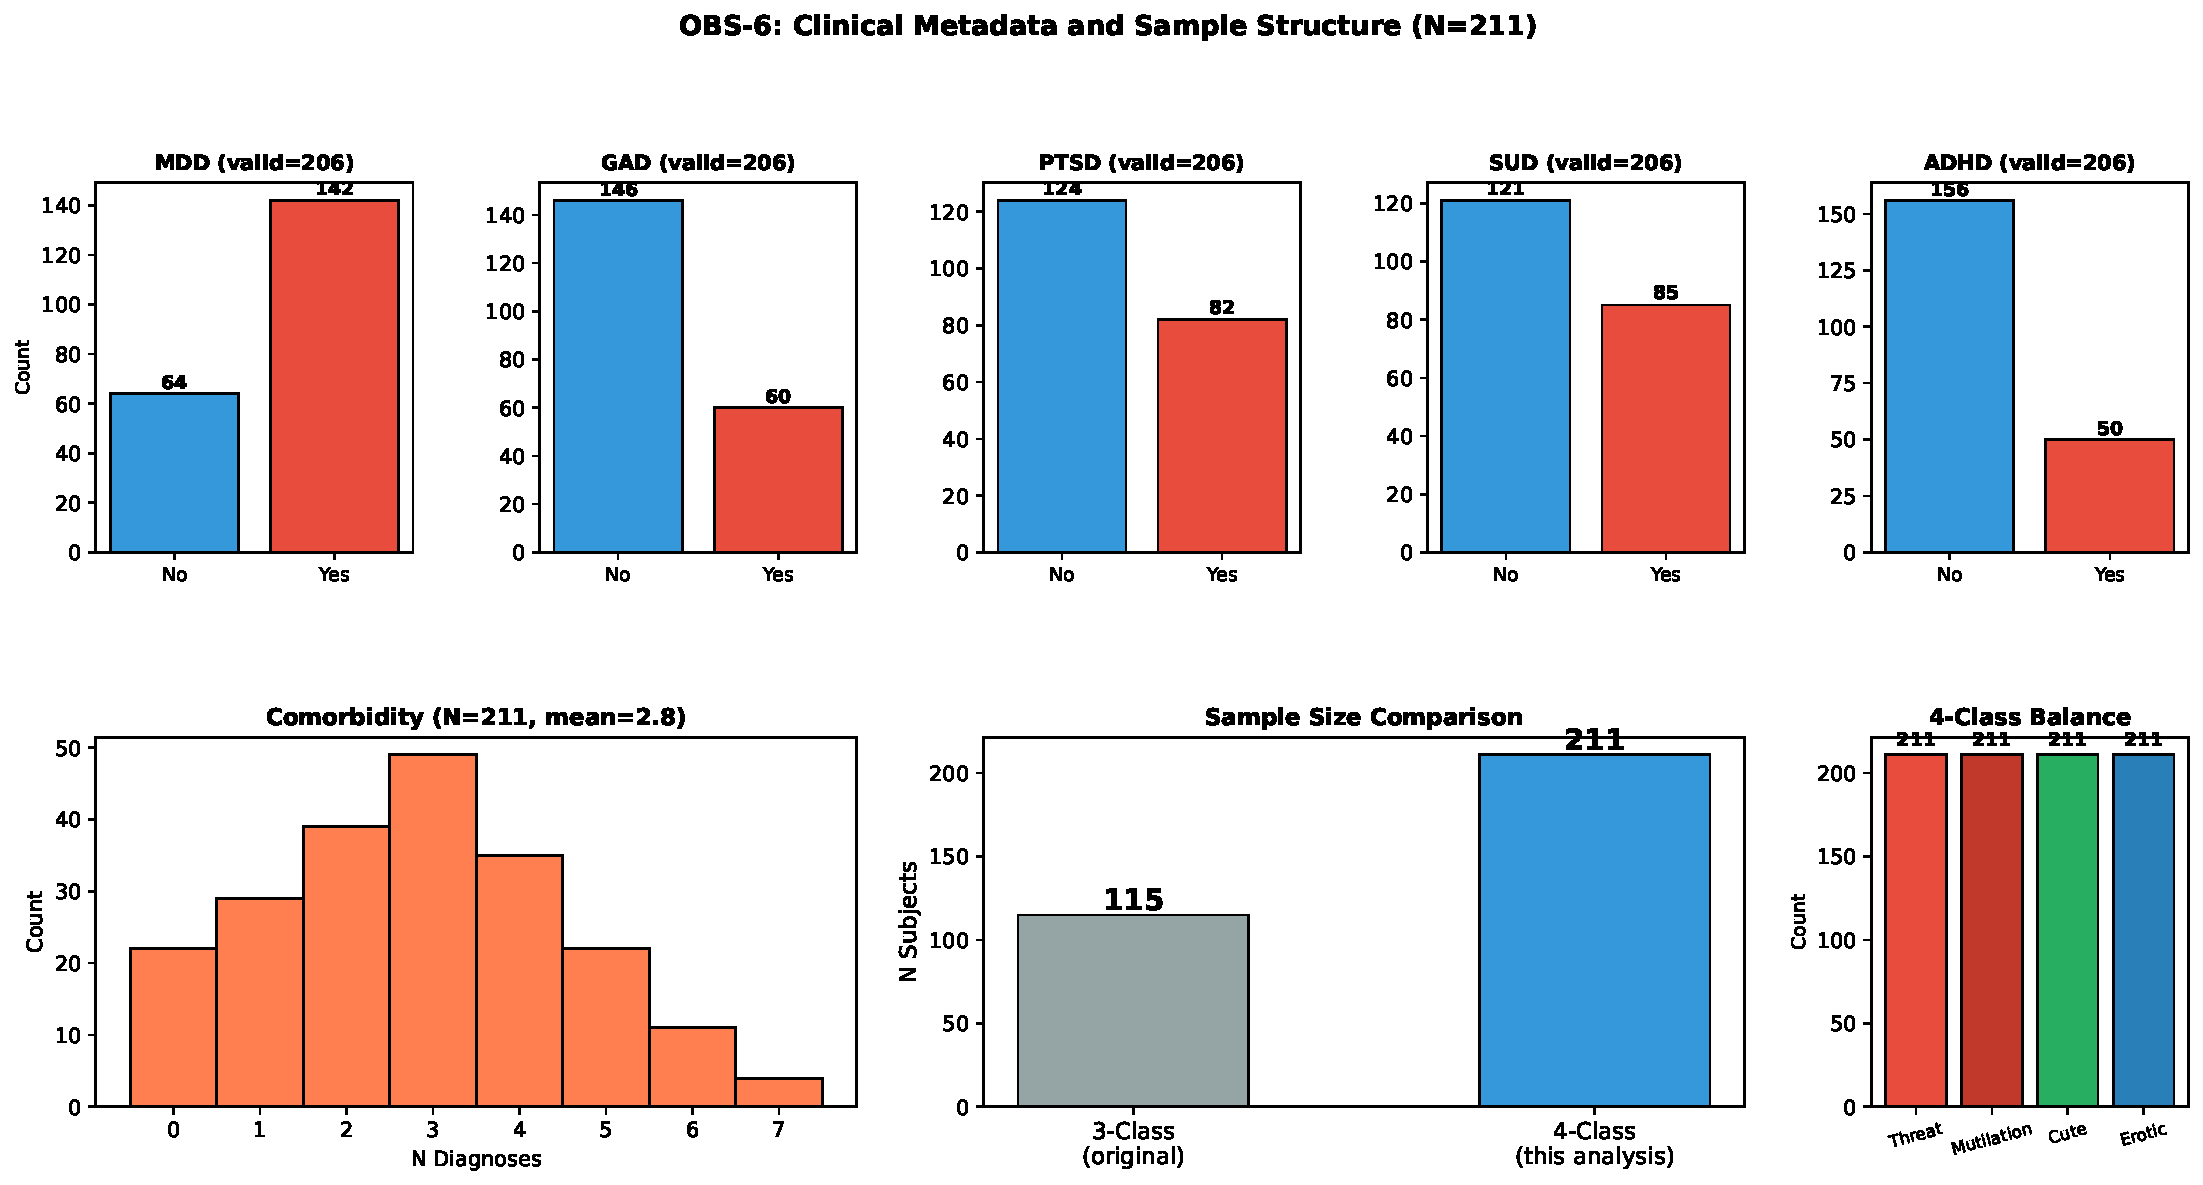
\includegraphics[width=\textwidth]{pictures/appendixA/ch5_4class_obs06_clinical.pdf}
    \caption{Clinical metadata coverage for the four-class analysis ($N = 211$ subjects, $844$ observations). Group sizes and diagnostic distributions are identical to the three-class analysis because the same subjects contribute to both granularities.}
    \label{fig:app_4class_obs06}
\end{figure}

\begin{figure}[H]
    \centering
    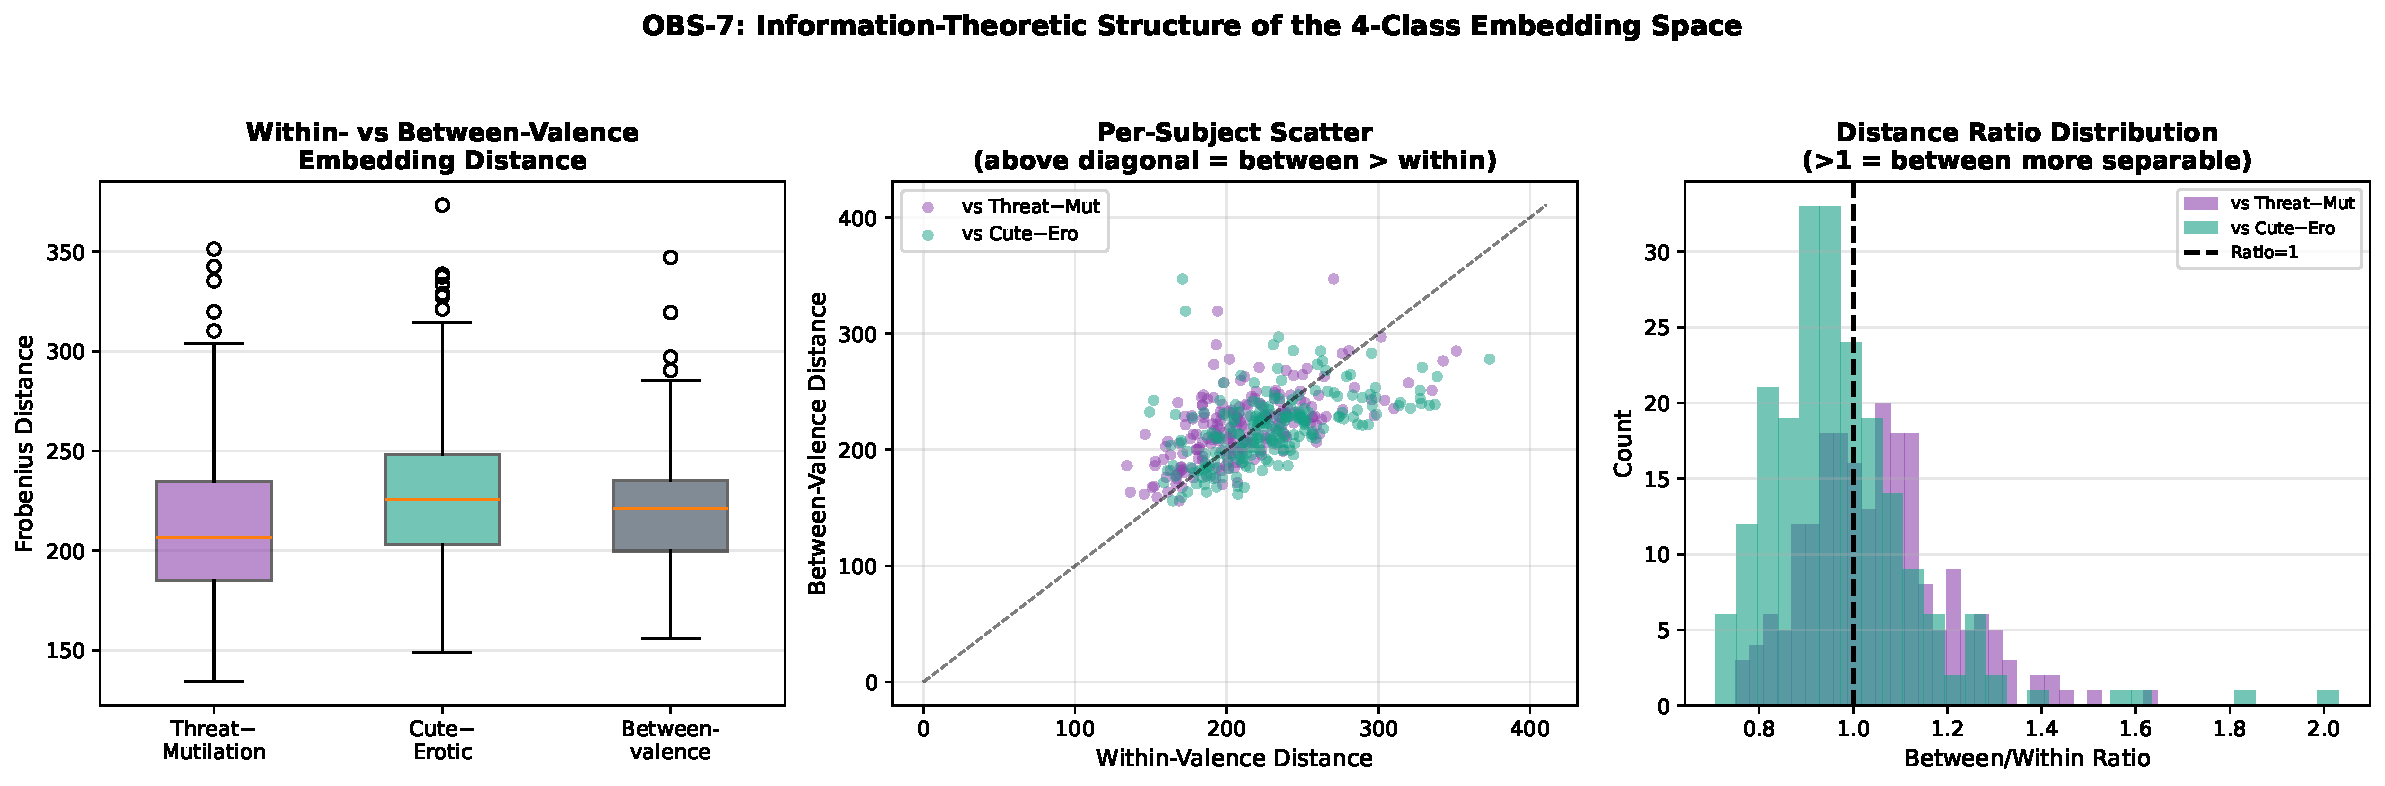
\includegraphics[width=\textwidth]{pictures/appendixA/ch5_4class_obs07_distance_structure.pdf}
    \caption{Archived pairwise distances in the four-category embedding. Threat--Mutilation and Cute--Erotic are grouped as ``within-valence'' in the display. Stimulus-level ratings and potential confounds were not modeled, so the observed distance ordering does not isolate valence or arousal.}
    \label{fig:app_4class_obs07}
\end{figure}


%% ═══════════════════════════════════════════════════════════════
%% SECTION A.2: FOUR-CLASS EXPERIMENTAL RESULTS
%% ═══════════════════════════════════════════════════════════════
\section{Four-Class Classification and Clinical Results}
\label{app:4class}

The following nine figures preserve the archived four-category results discussed in Chapter~\ref{chap:arspi_net}, Section~\ref{sec:ch5_4class}. Their PCA-dependent classification values are descriptive legacy estimates.

\begin{figure}[H]
    \centering
    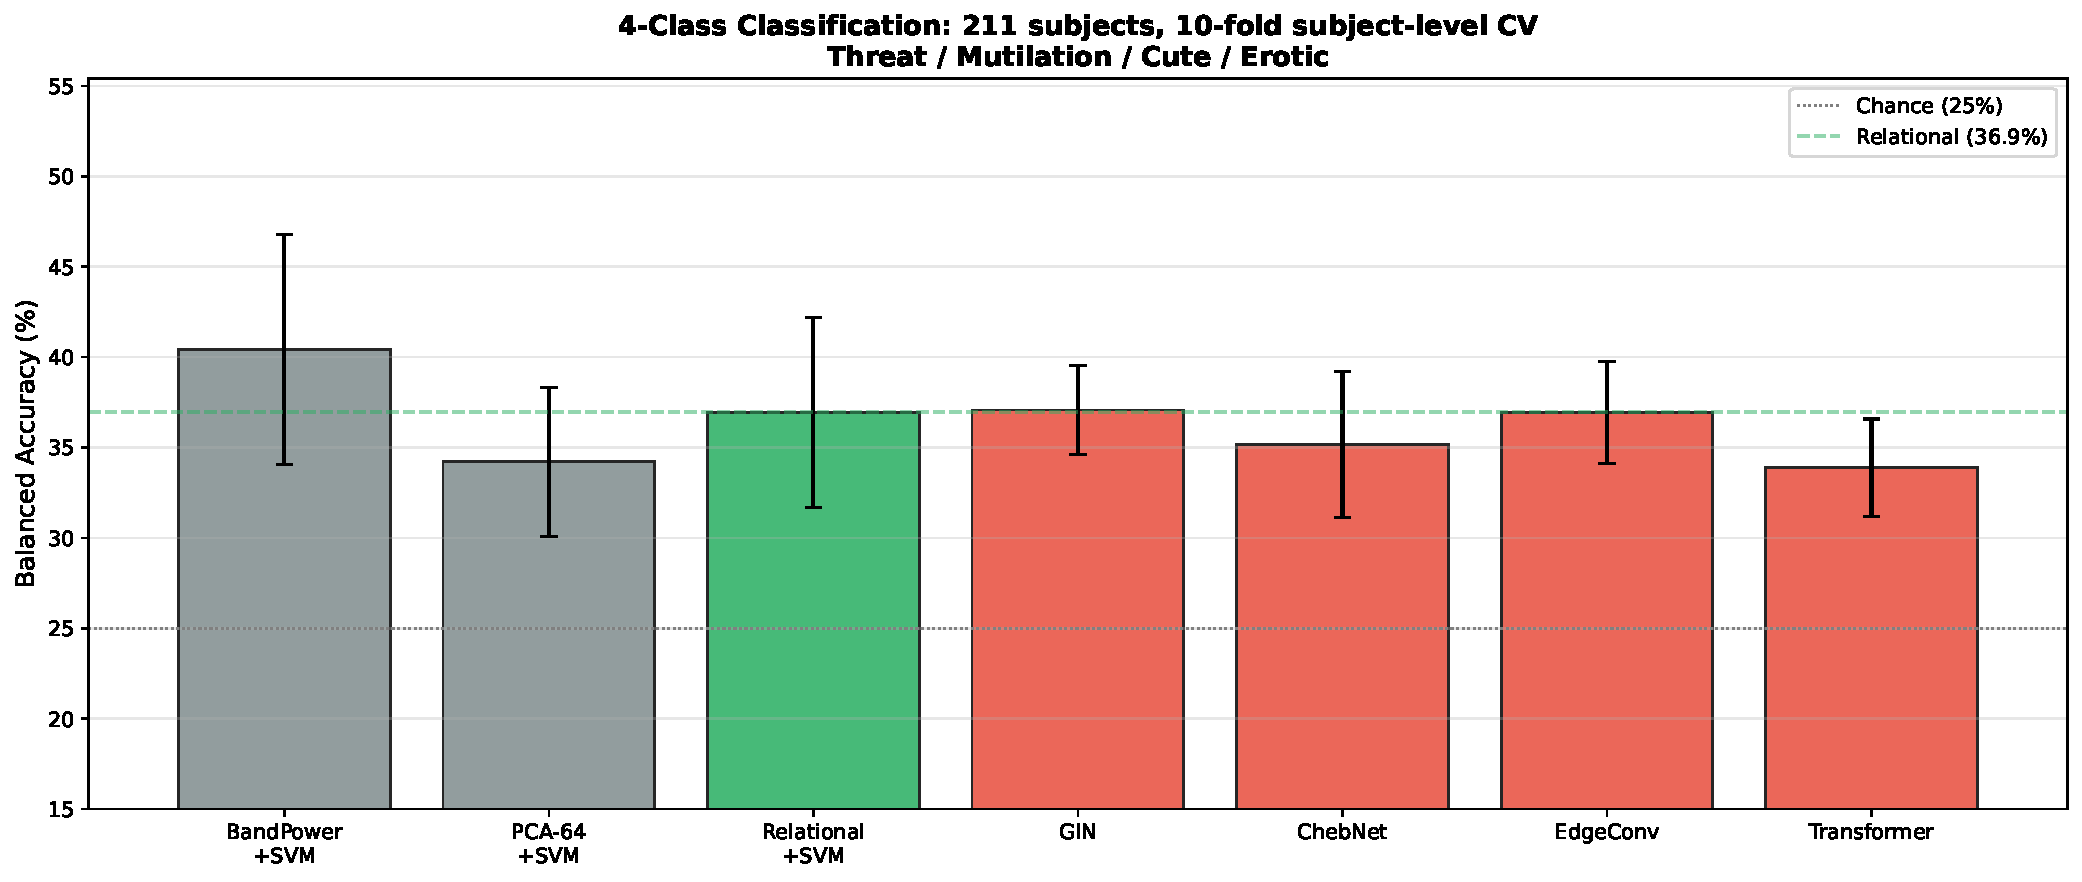
\includegraphics[width=\textwidth]{pictures/appendixA/ch5_4class_fig01_gnn_comparison.pdf}
    \caption{Archived four-category classification comparison ($N=211$, 844 observations). Band-power is 40.4\% and the reservoir embedding 34.2\%. The unmatched three- and four-condition pipelines do not support a replication or regime-boundary claim.}
    \label{fig:app_4class_fig01}
\end{figure}

\begin{figure}[H]
    \centering
    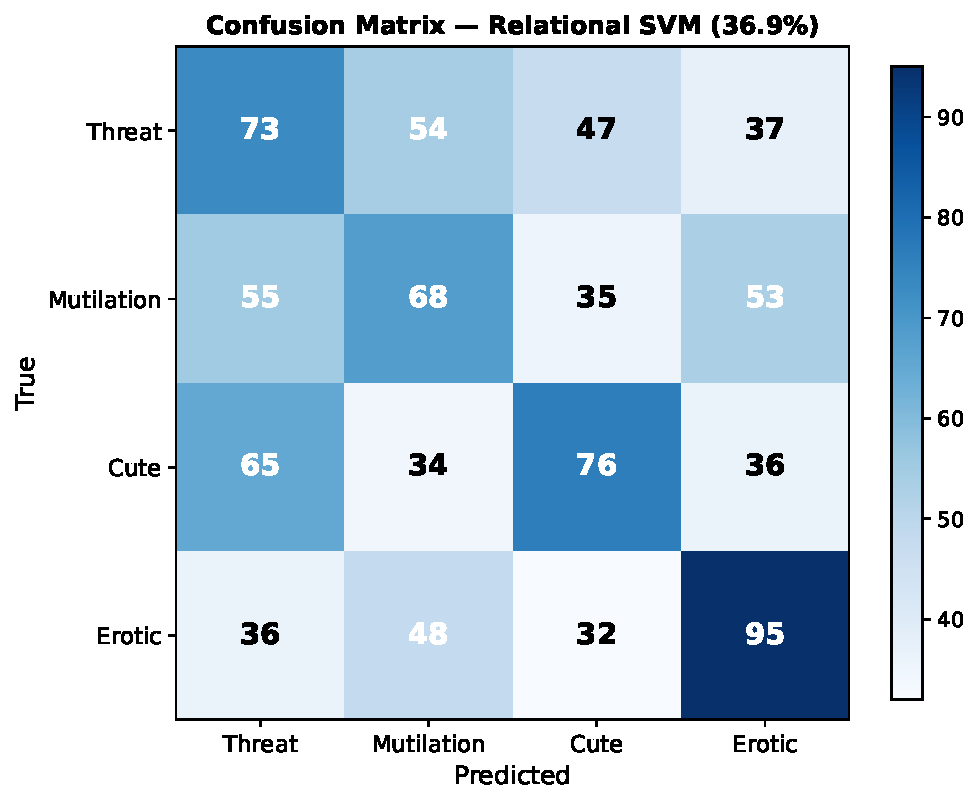
\includegraphics[width=\textwidth]{pictures/appendixA/ch5_4class_fig02_confusion_matrix.pdf}
    \caption{Archived four-category confusion matrix. Threat$\leftrightarrow$Mutilation and Cute$\leftrightarrow$Erotic errors account for $33\%$ of misclassifications. This error count does not by itself establish a valence-organized geometry.}
    \label{fig:app_4class_fig02}
\end{figure}

\begin{figure}[H]
    \centering
    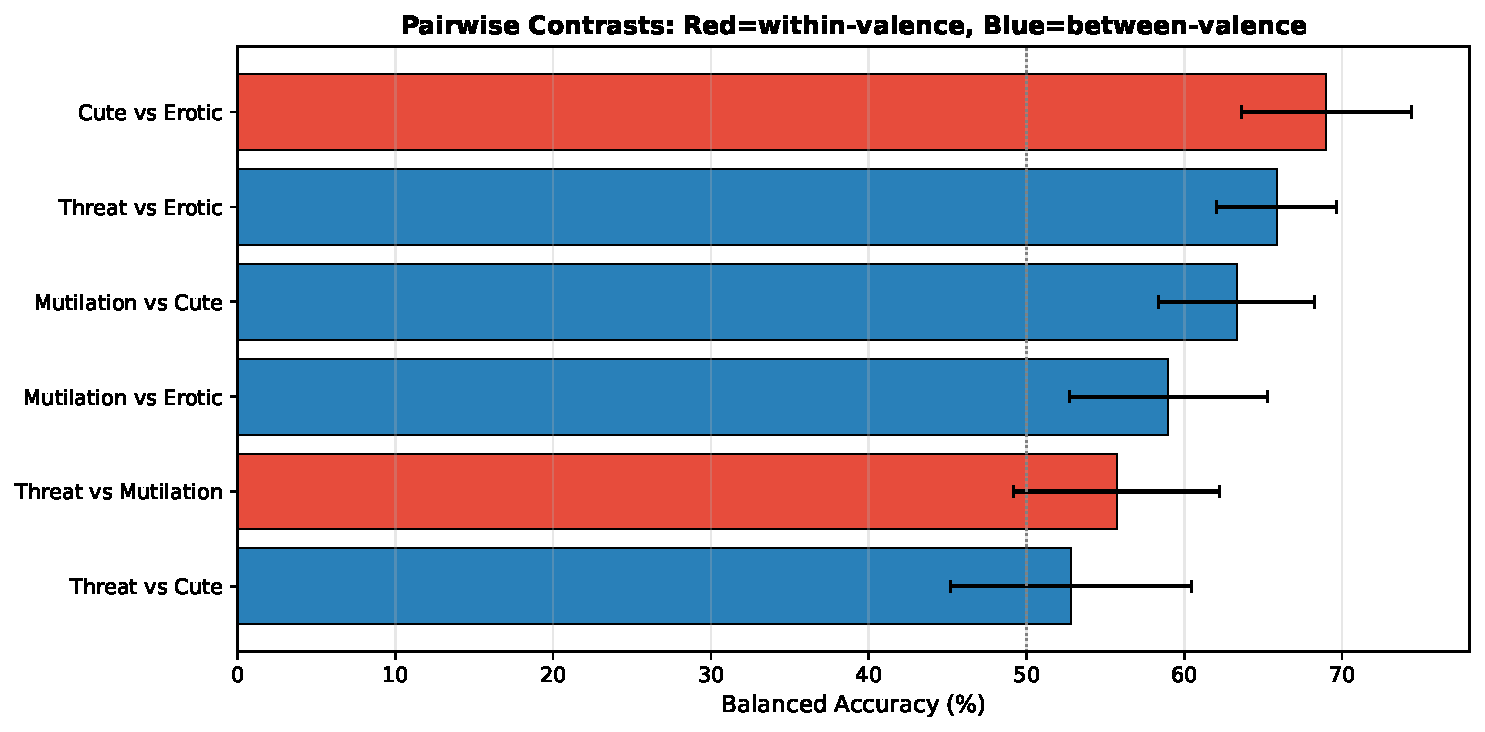
\includegraphics[width=\textwidth]{pictures/appendixA/ch5_4class_fig03_pairwise_contrasts.pdf}
    \caption{Archived pairwise four-category accuracies. Cute versus Erotic is highest (69.0\%) and Threat versus Cute lowest (52.8\%). Because stimulus-level arousal and valence scores were not modeled and the contrasts differ in multiple properties, the ranking does not isolate an arousal effect.}
    \label{fig:app_4class_fig03}
\end{figure}

\begin{figure}[H]
    \centering
    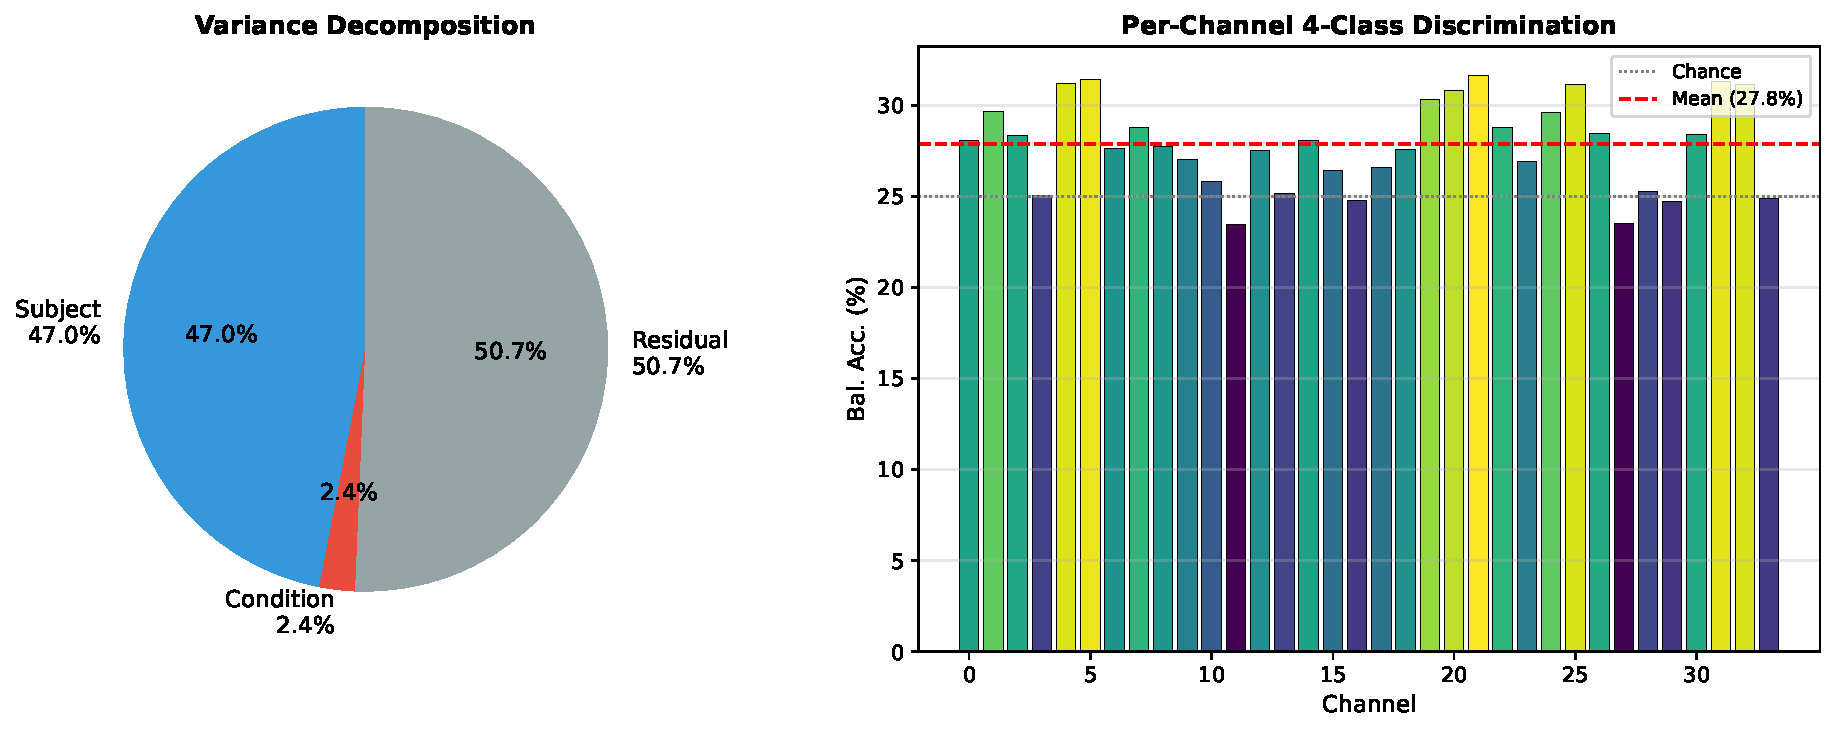
\includegraphics[width=\textwidth]{pictures/appendixA/ch5_4class_fig04_variance_channels.pdf}
    \caption{Archived sums-of-squares decomposition and per-channel analysis at four-category resolution. Participant, category, and residual fractions are $47.0\%$, $2.4\%$, and $50.7\%$, respectively. The unmatched three-condition fractions are shown for context, not as an independent replication.}
    \label{fig:app_4class_fig04}
\end{figure}

\begin{figure}[H]
    \centering
    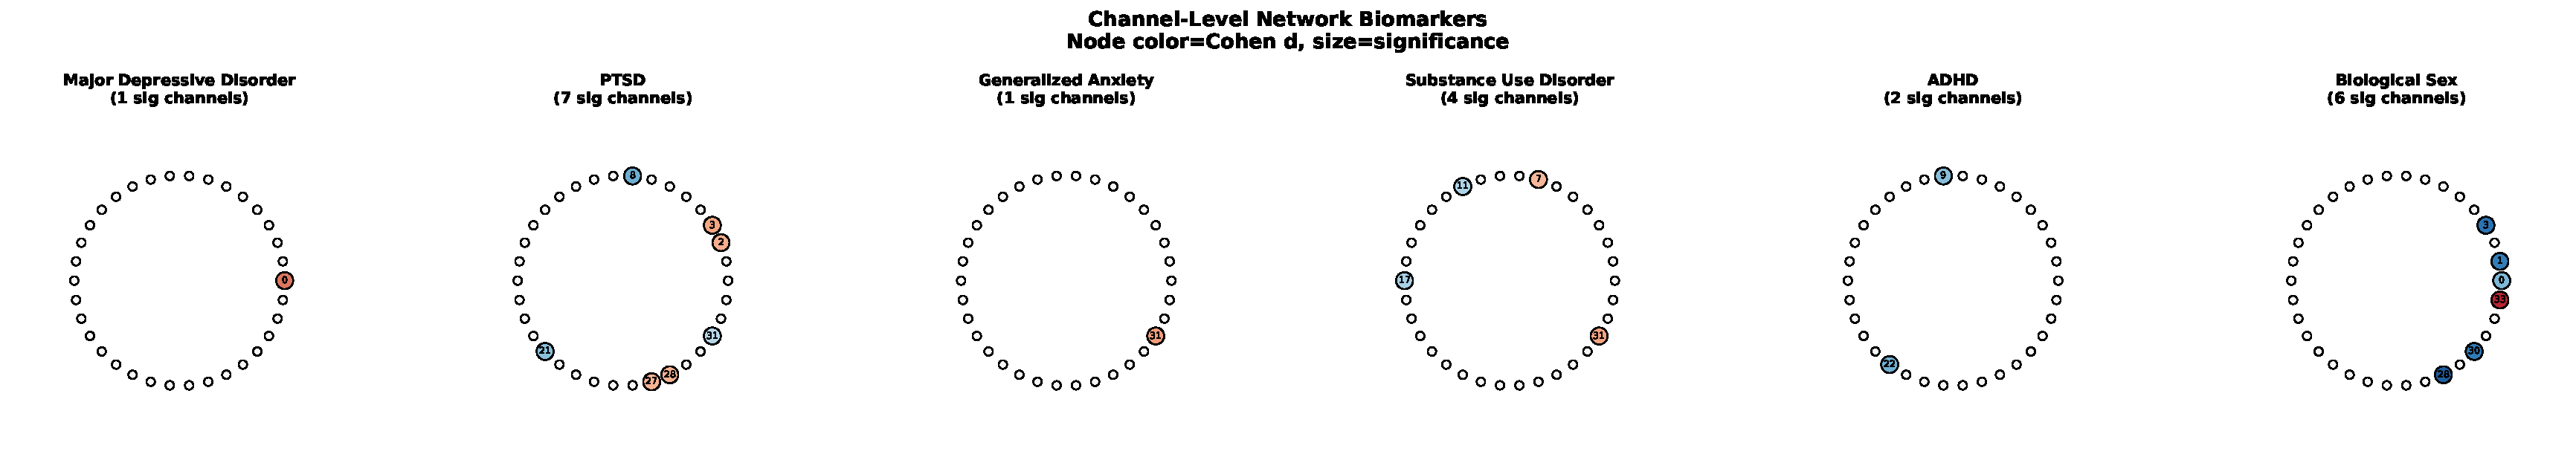
\includegraphics[width=\textwidth]{pictures/appendixA/ch5_4class_fig05_channel_biomarkers.pdf}
    \caption{Uncorrected four-category channel--metric clinical screens. Eleven PTSD cells have nominal $p<0.05$; these are not biomarkers, do not establish disorder-specific spatial signatures, and require correction and external replication.}
    \label{fig:app_4class_fig05}
\end{figure}

\begin{figure}[H]
    \centering
    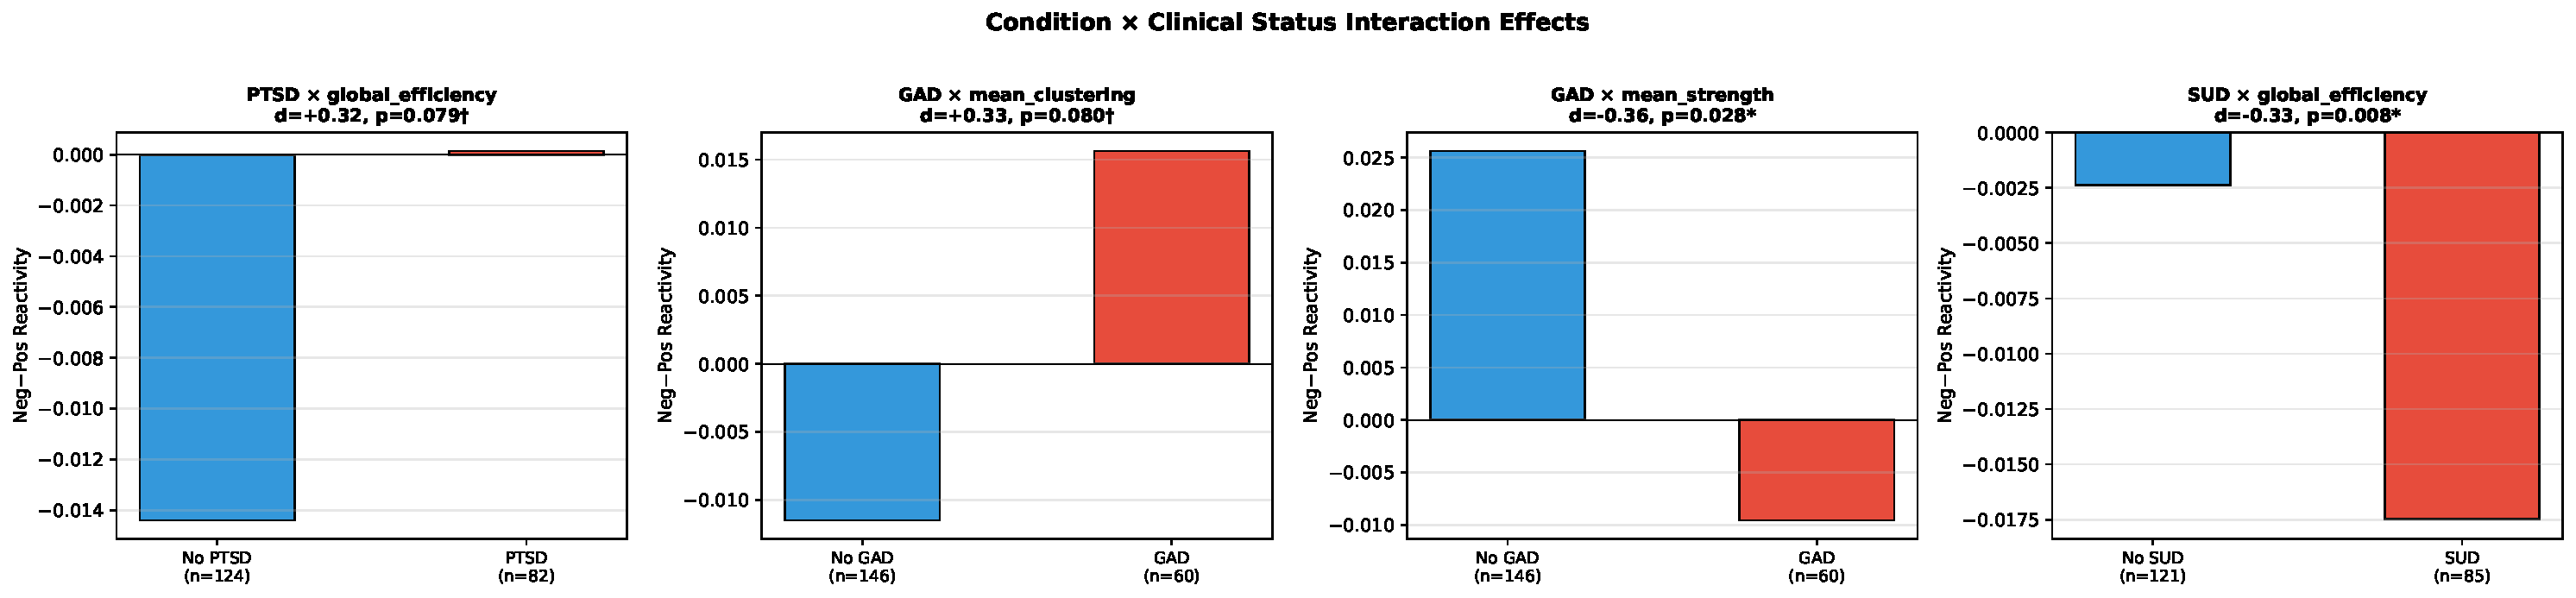
\includegraphics[width=\textwidth]{pictures/appendixA/ch5_4class_fig06_interactions.pdf}
    \caption{Exploratory condition-by-clinical interactions. PTSD by Threat--Mutilation has uncorrected $p=0.036$, and SUD by global efficiency has $p=0.008$ in this pipeline. Neither result is a corrected, independent replication or evidence of network reorganization.}
    \label{fig:app_4class_fig06}
\end{figure}

\begin{figure}[H]
    \centering
    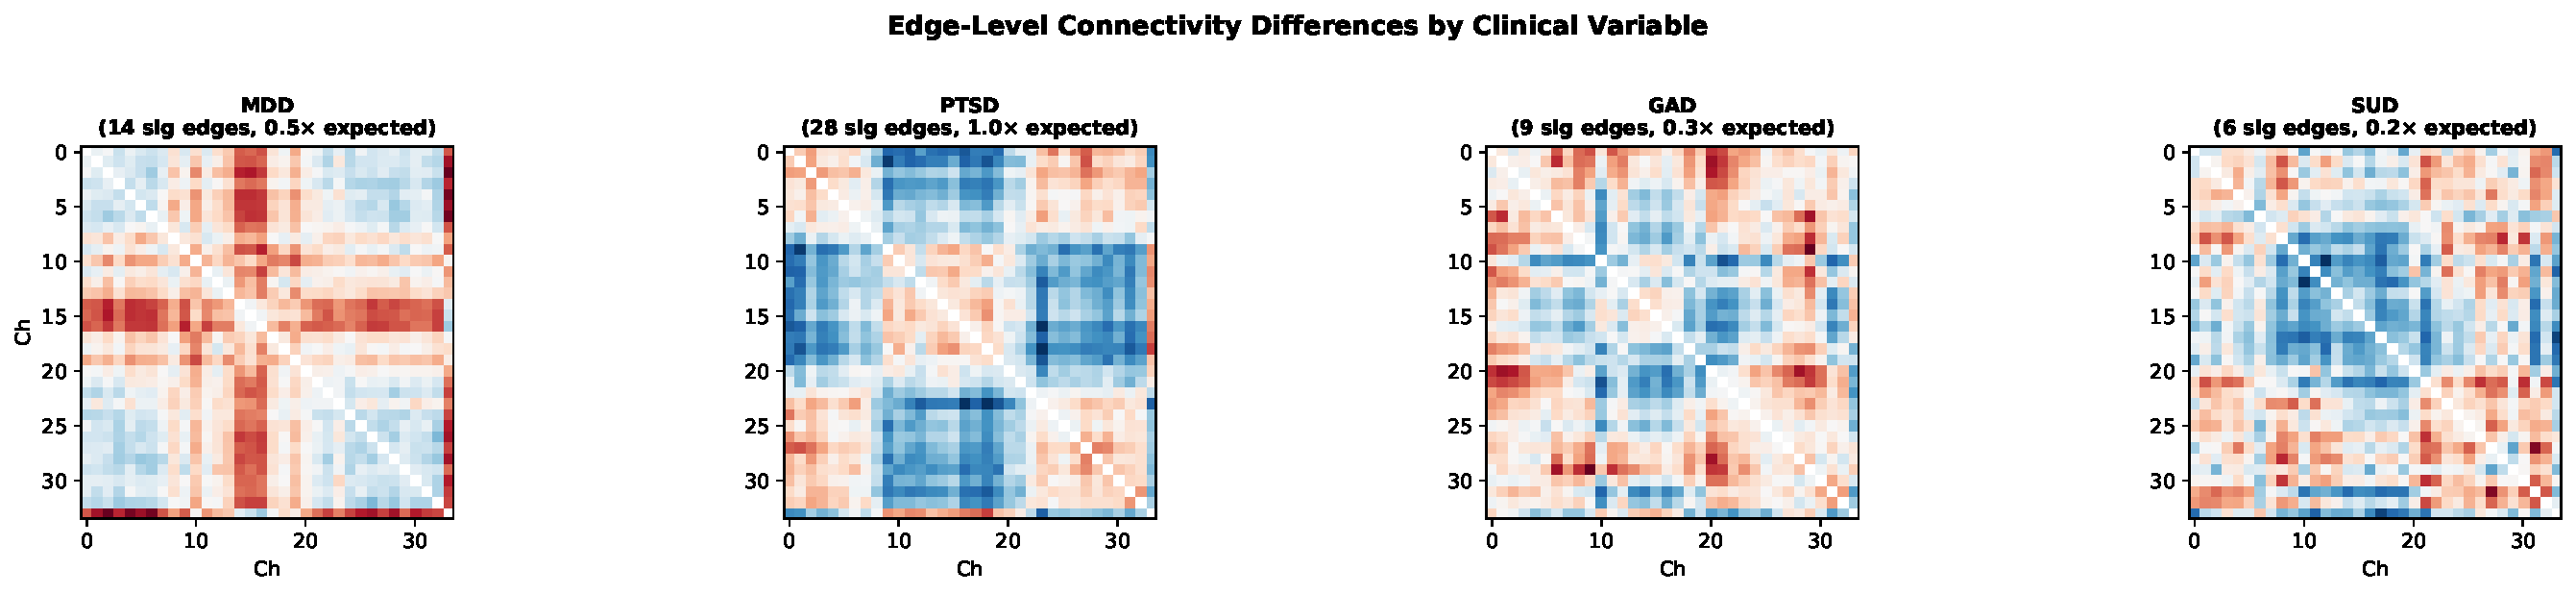
\includegraphics[width=\textwidth]{pictures/appendixA/ch5_4class_fig07_edge_biomarkers.pdf}
    \caption{Four-category edge-level screens. Twenty-eight PTSD edges have nominal significance in the archived analysis; the figure does not establish biomarkers or a granularity effect.}
    \label{fig:app_4class_fig07}
\end{figure}

\begin{figure}[H]
    \centering
    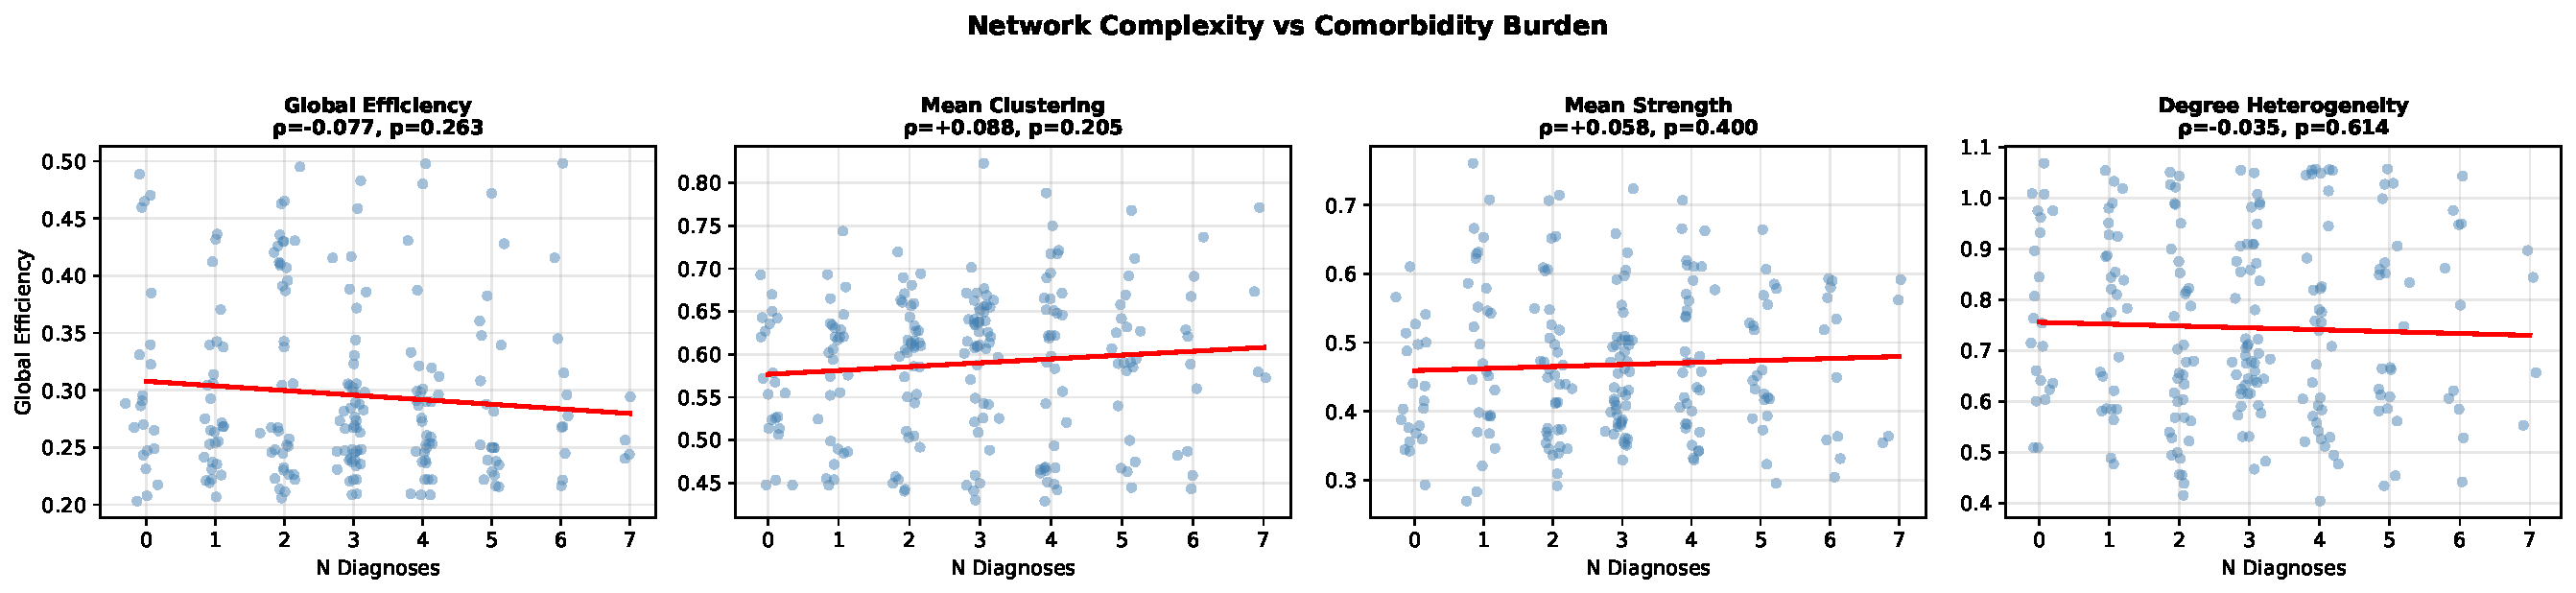
\includegraphics[width=\textwidth]{pictures/appendixA/ch5_4class_fig08_comorbidity.pdf}
    \caption{Comorbidity-count comparisons with graph summaries. Non-significant correlations do not rule out confounding by comorbidity or other clinical variables.}
    \label{fig:app_4class_fig08}
\end{figure}

\begin{figure}[H]
    \centering
    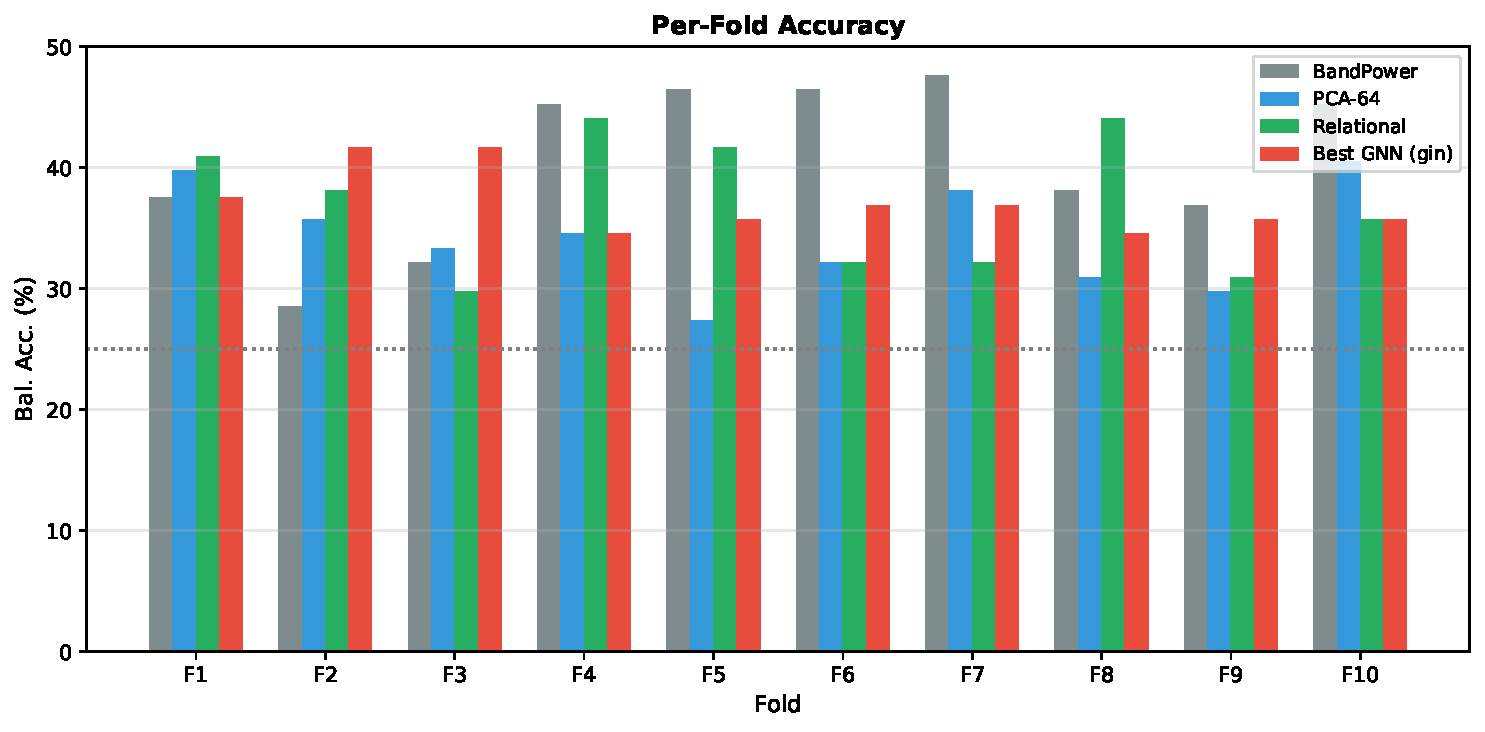
\includegraphics[width=\textwidth]{pictures/appendixA/ch5_4class_fig09_fold_comparison.pdf}
    \caption{Archived per-fold accuracies for band-power, reservoir, and graph classifiers. Folds overlap in training data and do not supply independent evidence of robustness.}
    \label{fig:app_4class_fig09}
\end{figure}


%% ═══════════════════════════════════════════════════════════════
%% SECTION A.3: LAYER ABLATION FIGURES
%% ═══════════════════════════════════════════════════════════════
\section{Layer Ablation and Complementarity Figures}
\label{app:ablation}

The following three figures present the complete visualization of the layer ablation experiment reported in Chapter~\ref{chap:arspi_net}, Section~\ref{sec:ch5_ablation}. The numerical results are presented in Tables~\ref{tab:emotion_ablation} and~\ref{tab:clinical_ablation} in the main text.

\begin{figure}[H]
    \centering
    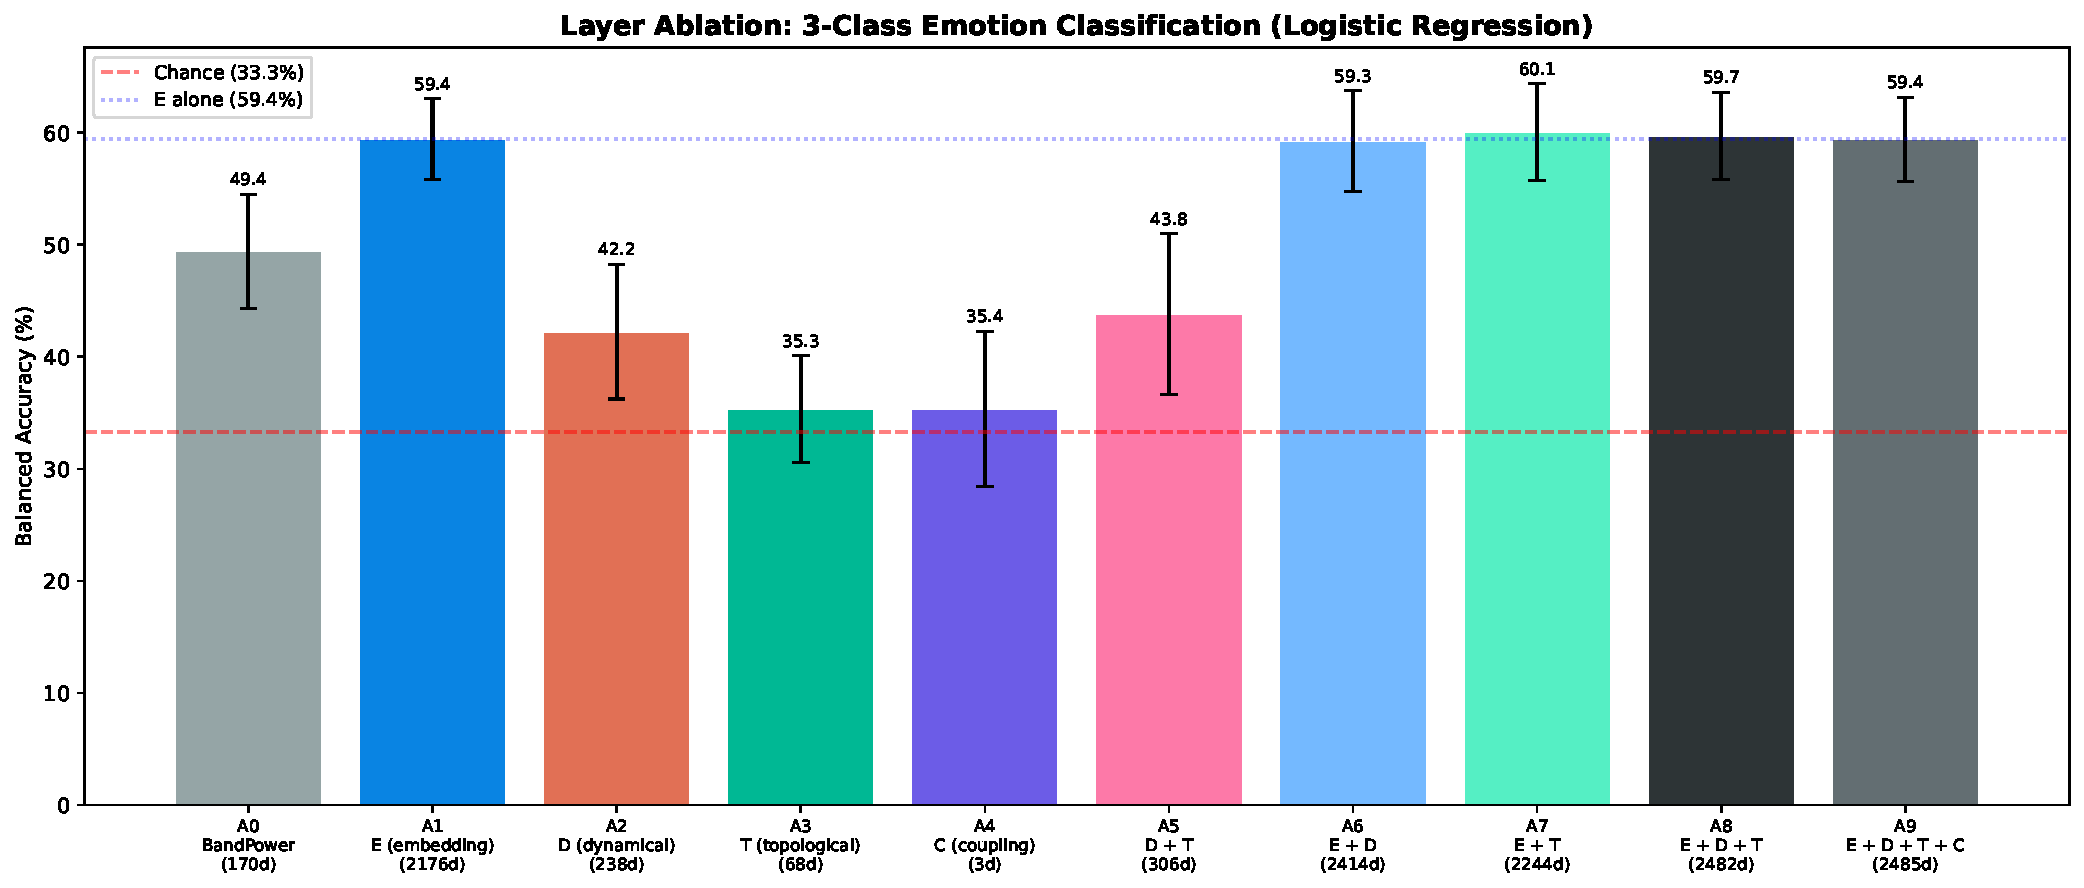
\includegraphics[width=\textwidth]{pictures/appendixA/ch5_fig_emotion_ablation.pdf}
    \caption{Archived three-condition layer comparison (logistic regression, 10 subject-grouped folds). A0: band-power ($49.4\%$); A1: embedding ($59.4\%$); A2: dynamical summaries ($42.2\%$); A3: topological summaries ($35.3\%$); A4: coupling ($35.4\%$); A5--A9: combinations. A1 has the highest recorded mean, and no combination exceeds it by more than $0.7$ percentage points. Fold standard deviations are descriptive because training sets overlap.}
    \label{fig:app_emotion_ablation}
\end{figure}

\begin{figure}[H]
    \centering
    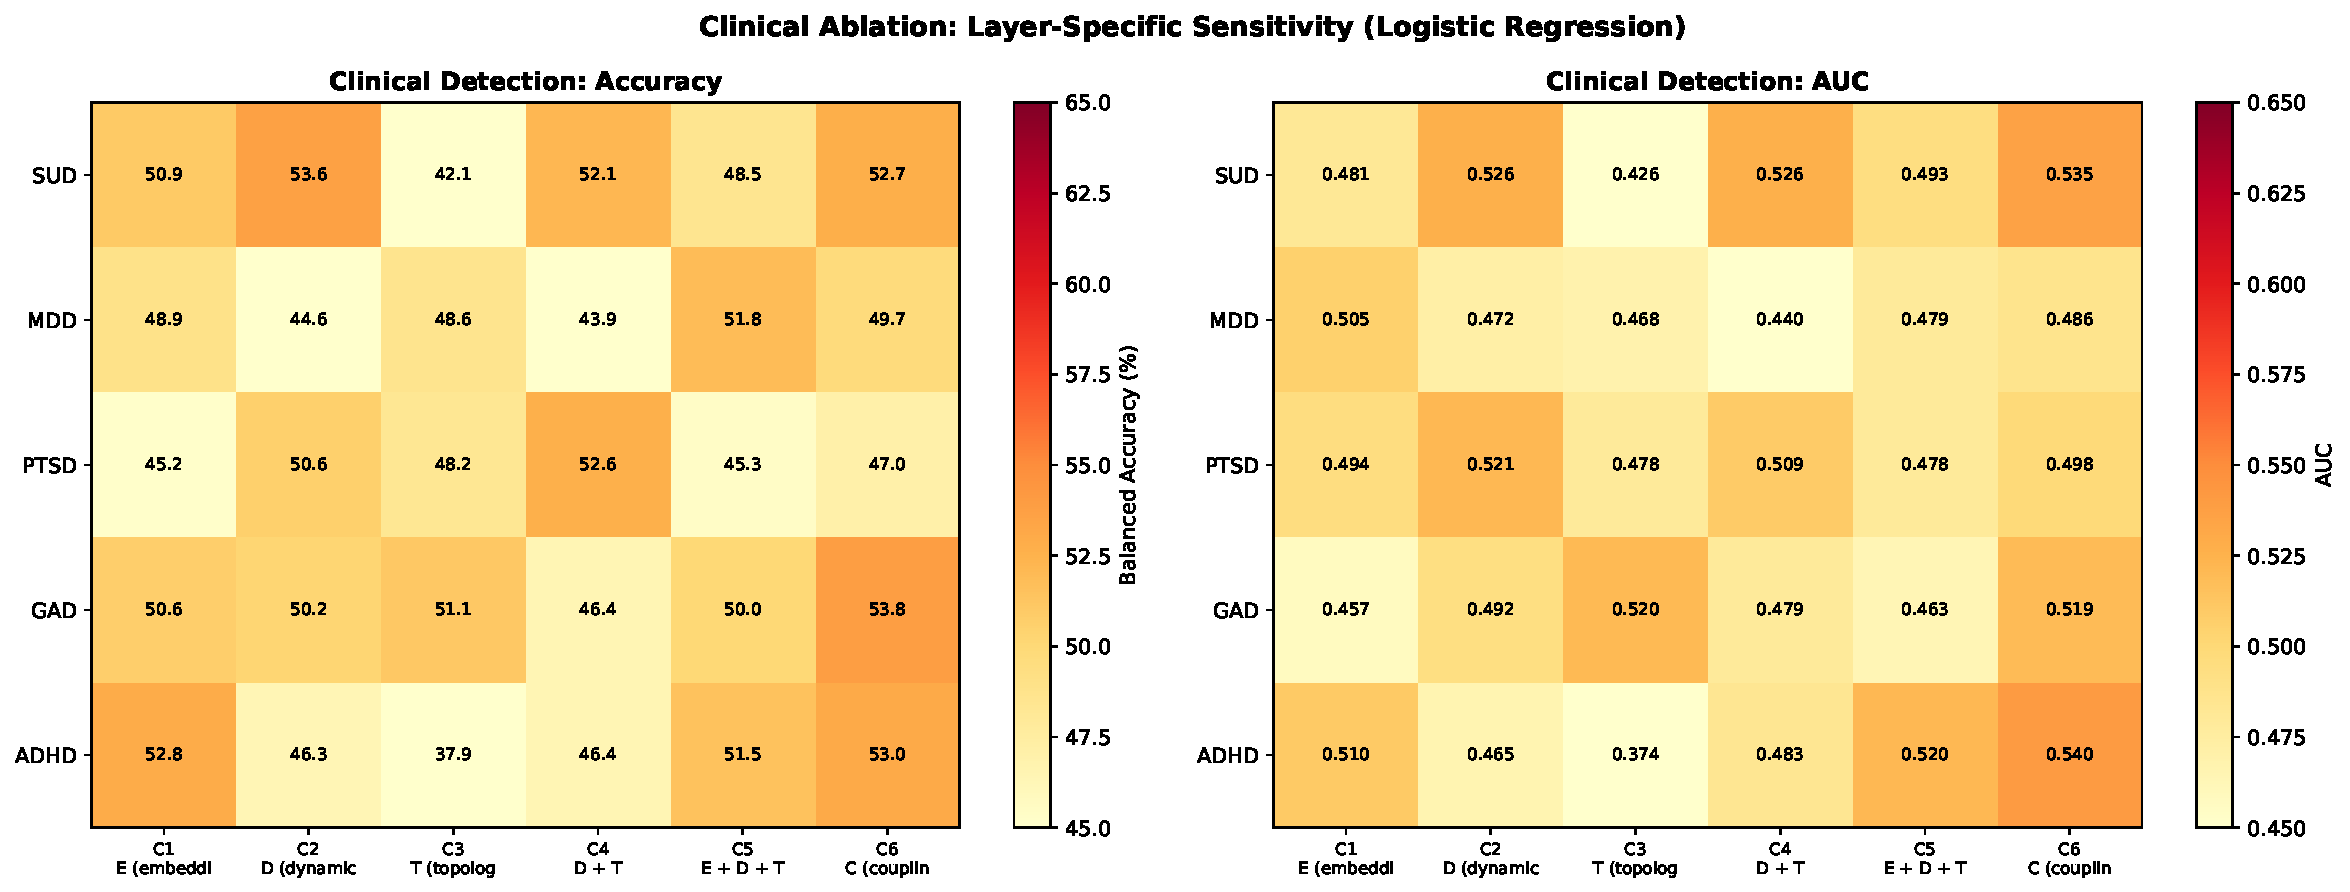
\includegraphics[width=\textwidth]{pictures/appendixA/ch5_fig_clinical_ablation.pdf}
    \caption{Exploratory subject-level five-fold clinical readouts by feature block. The post-hoc maximum differs by label, but near-chance performance and model selection prevent a disorder- or layer-specific claim.}
    \label{fig:app_clinical_ablation}
\end{figure}

\begin{figure}[H]
    \centering
    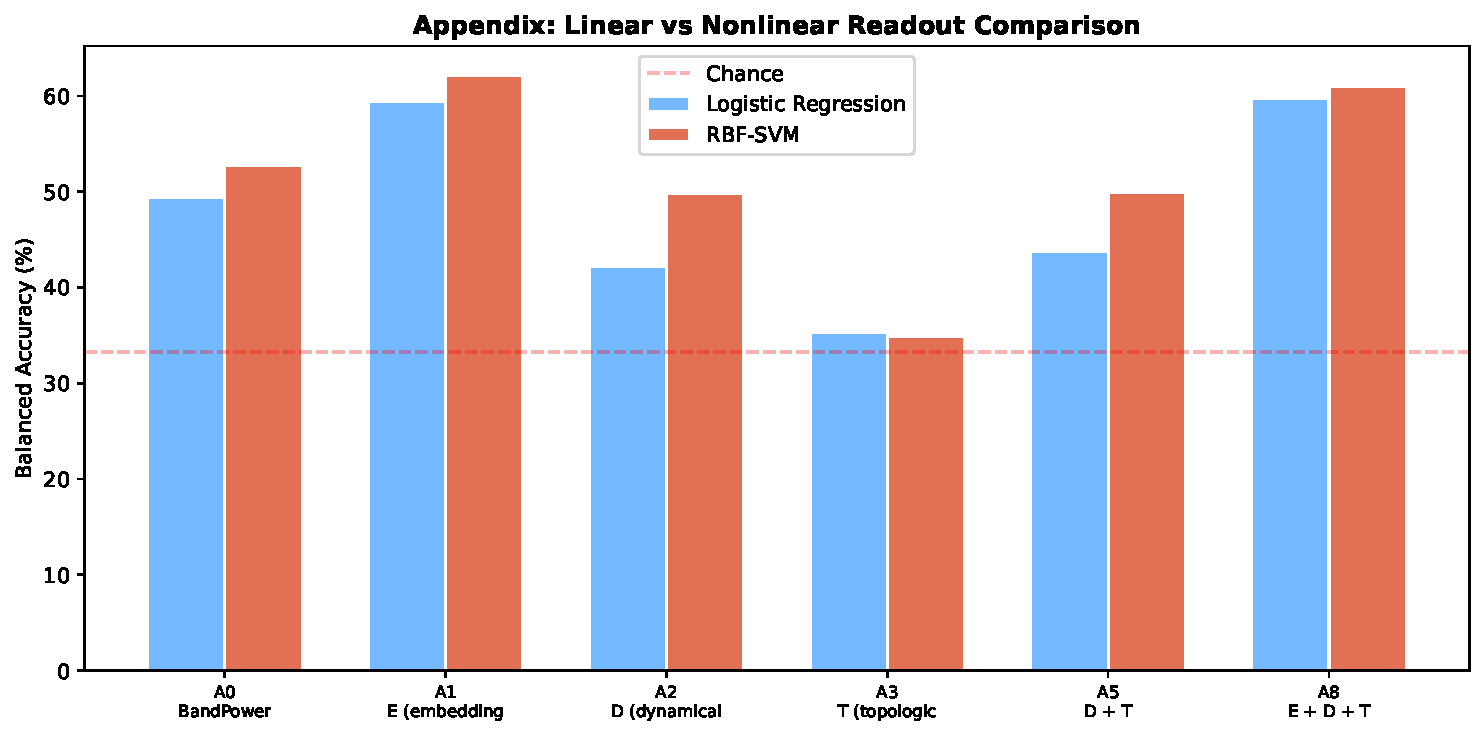
\includegraphics[width=\textwidth]{pictures/appendixA/ch5_fig_rbf_sensitivity.pdf}
    \caption{Archived linear (logistic regression) and nonlinear (RBF-SVM) readout comparison. The embedding mean changes from $59.4\%$ to $62.1\%$; the dynamical-summary mean changes from $42.2\%$ to $49.8\%$. These finite, post-hoc differences do not identify a uniquely nonlinear information source.}
    \label{fig:app_rbf_sensitivity}
\end{figure}


%% ═══════════════════════════════════════════════════════════════
%% SECTION A.4: CHAPTER 6 FIGURES
%% ═══════════════════════════════════════════════════════════════
\section{Chapter 6: Supplementary Raw Observations}
\label{app:ch6_figs}

The following eight archived figures display distributions, channel-index heterogeneity, population firing-rate summaries, within-epoch phase summaries, graph-derived quantities, and clinical metadata coverage. The seven experimental result figures (EXP-6.1 through EXP-6.7) are presented inline in Chapter~\ref{chap:dynamics}.

\begin{figure}[H]
    \centering
    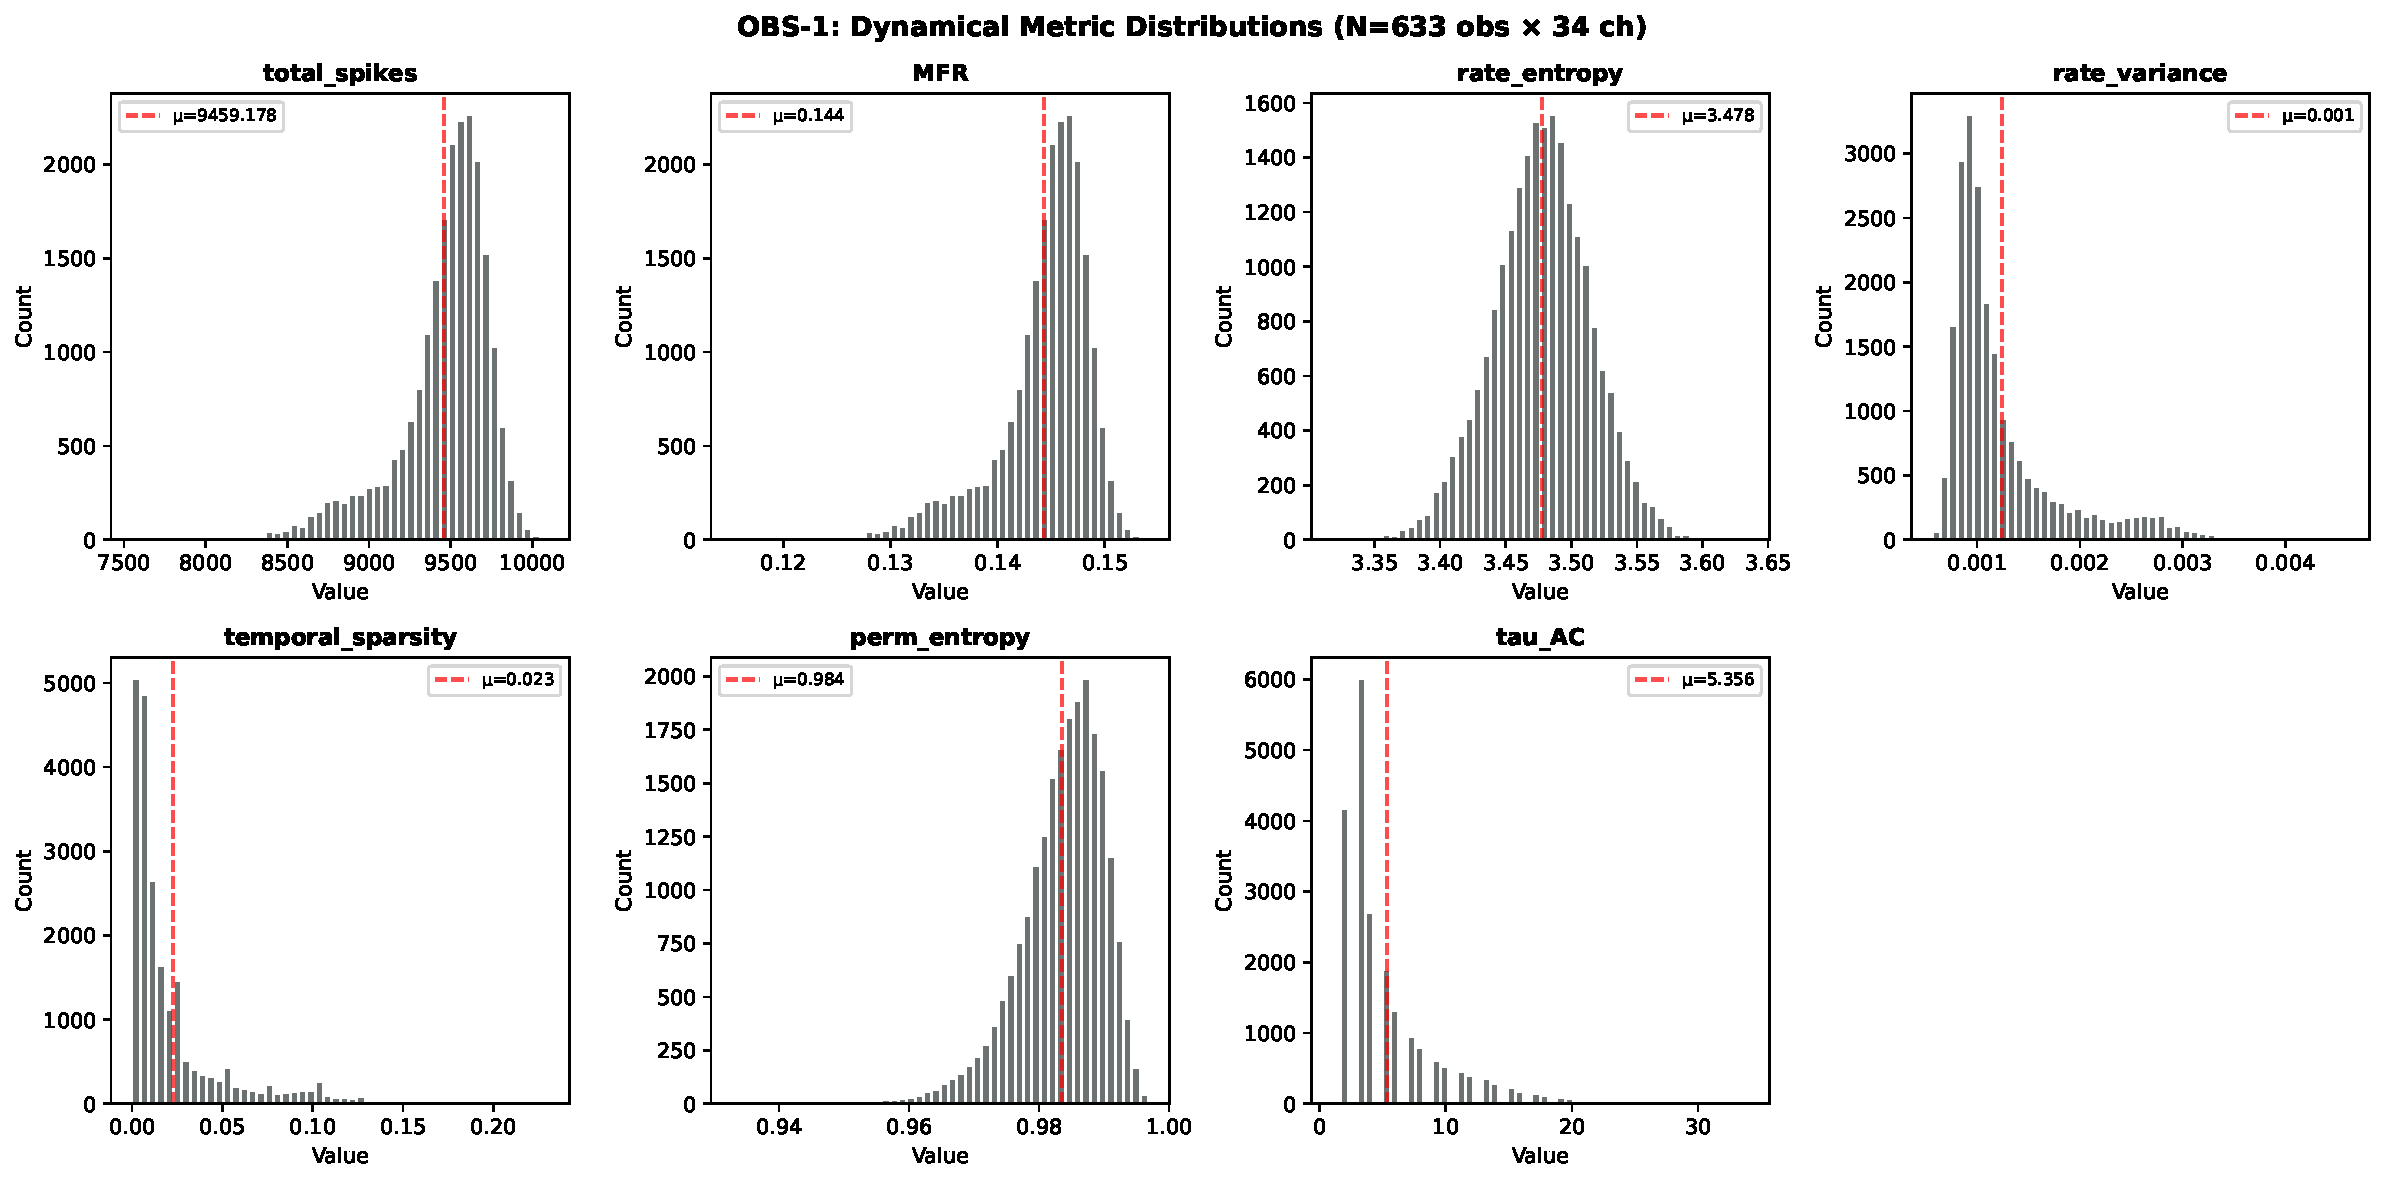
\includegraphics[width=\textwidth]{pictures/appendixA/obs01_metric_distributions.pdf}
    \caption{OBS-1: Dynamical metric distributions across all $633$ observations ($211$ subjects $\times$ $3$ conditions). Seven core metrics span different variability regimes: $\tau_{\text{AC}}$ (CV~$= 0.77$) and temporal sparsity (CV~$= 1.24$) show the highest variability; MFR (CV~$= 0.03$) and permutation entropy (CV~$= 0.007$) show the lowest.}
    \label{fig:app_ch6_obs01}
\end{figure}

\begin{figure}[H]
    \centering
    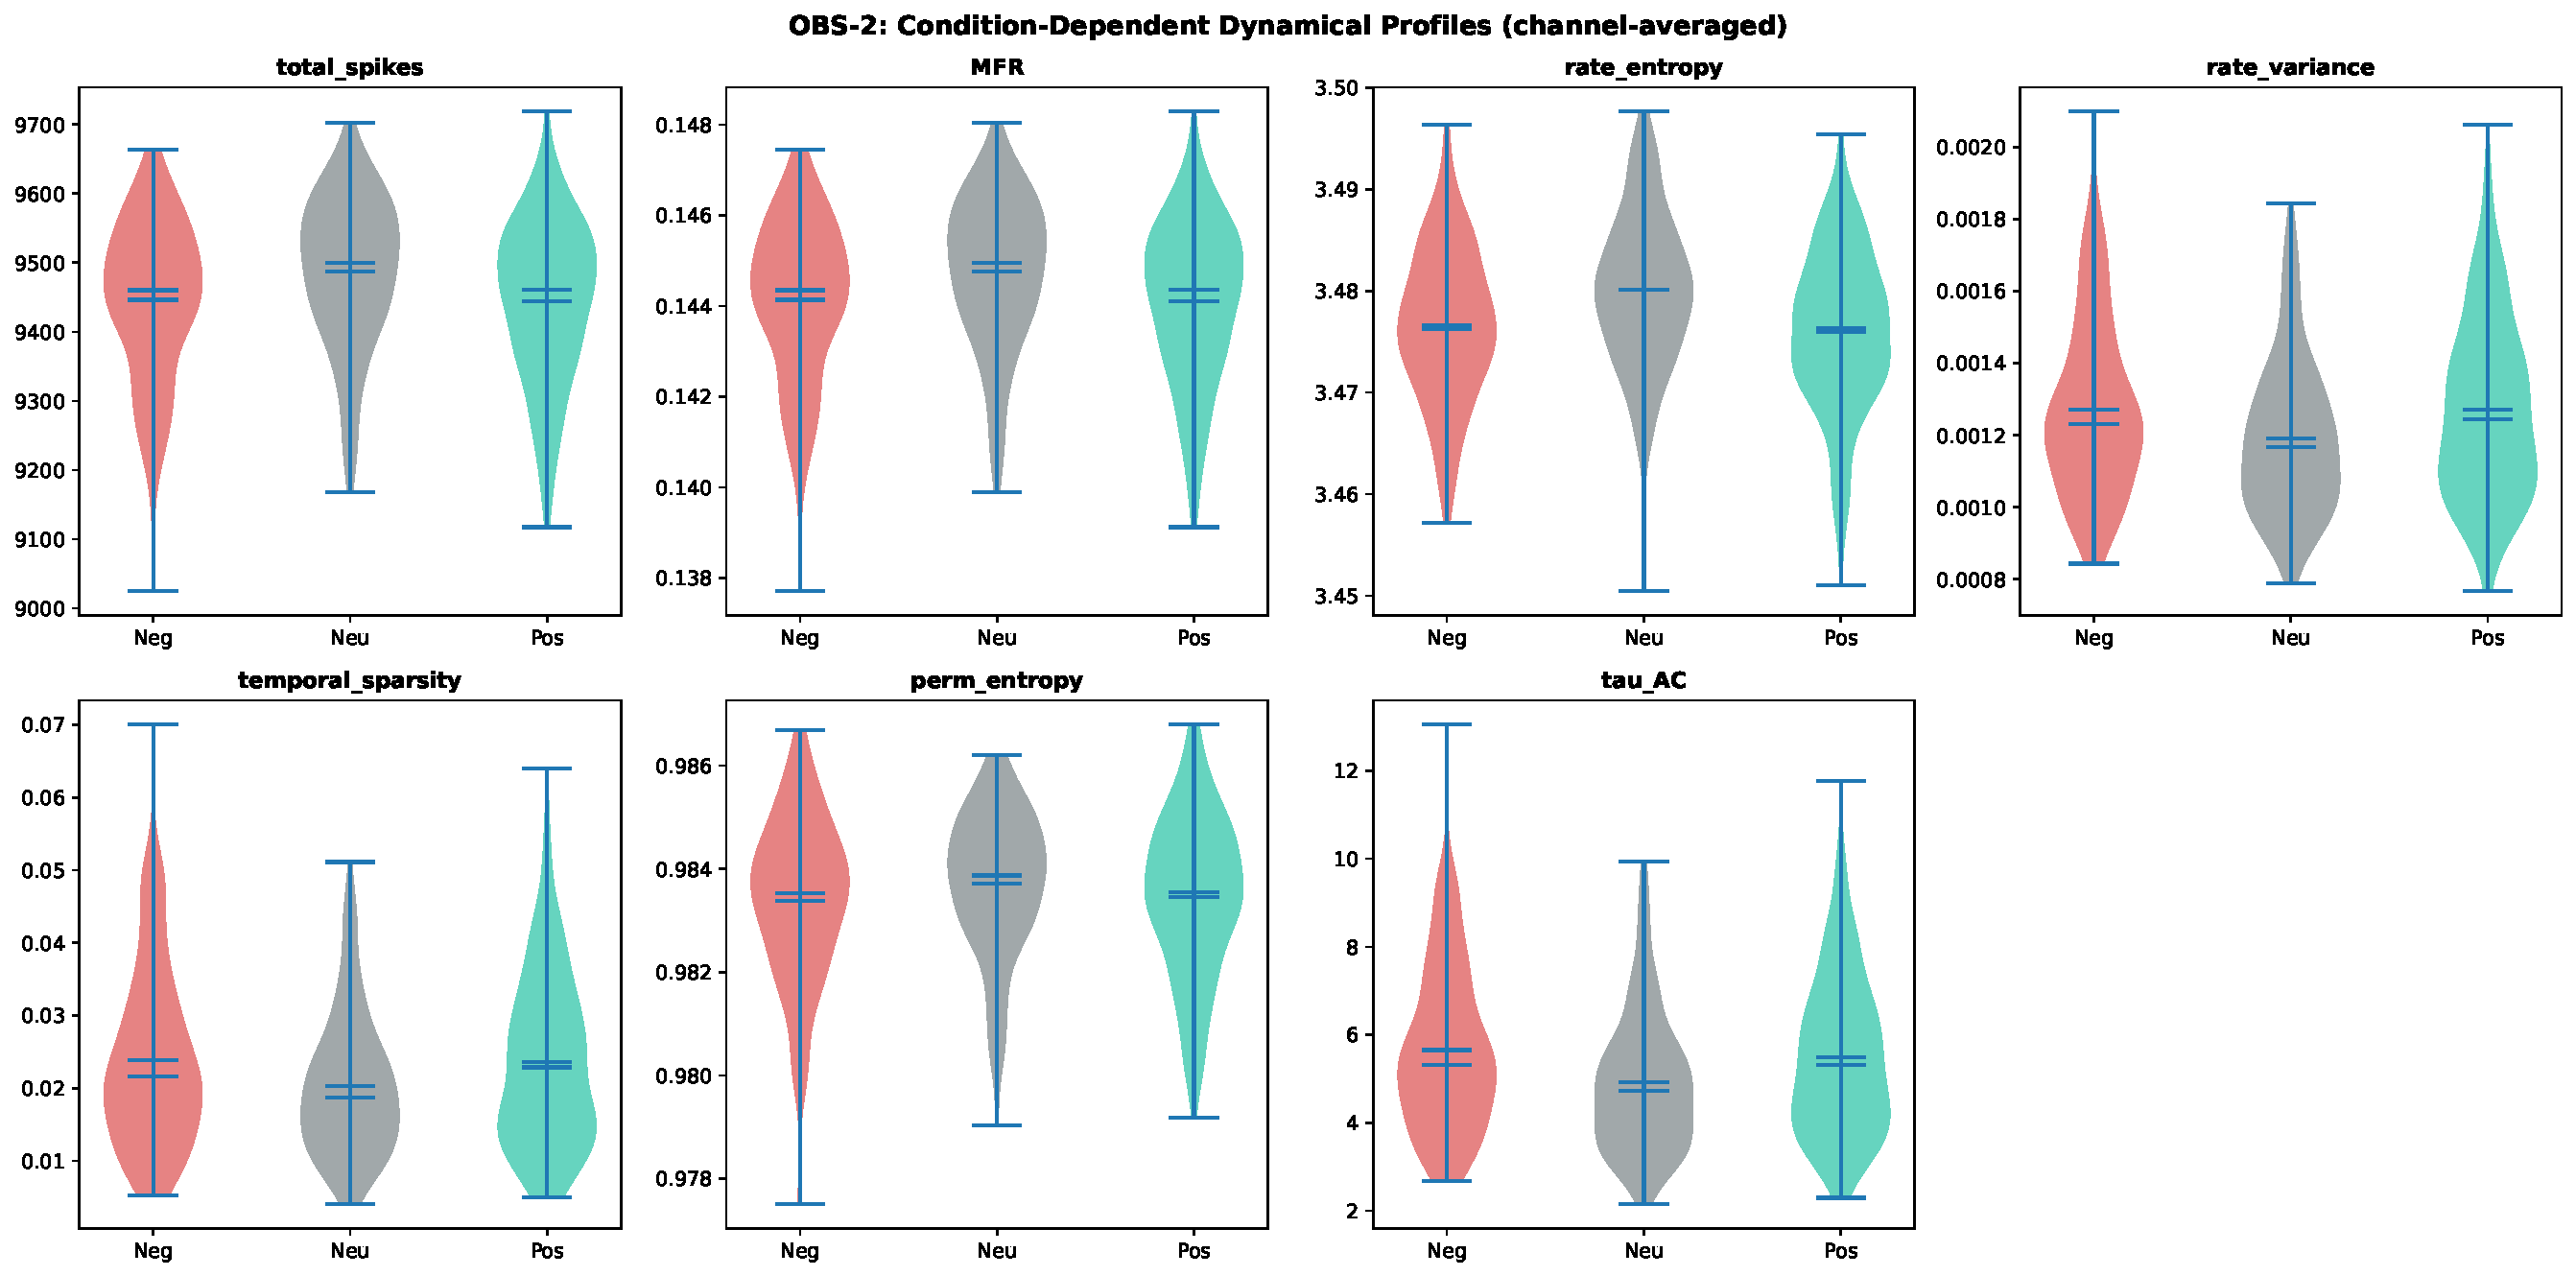
\includegraphics[width=\textwidth]{pictures/appendixA/obs02_condition_profiles.pdf}
    \caption{OBS-2: Archived condition-level dynamical summaries. Negative and Pleasant have similar means for the displayed metrics, while Neutral differs most for $\tau_{\text{AC}}$: Negative ($5.65$), Pleasant ($5.50$), and Neutral ($4.92$). No participant- or stimulus-level arousal scores were modeled, so the pattern cannot be attributed specifically to arousal.}
    \label{fig:app_ch6_obs02}
\end{figure}

\begin{figure}[H]
    \centering
    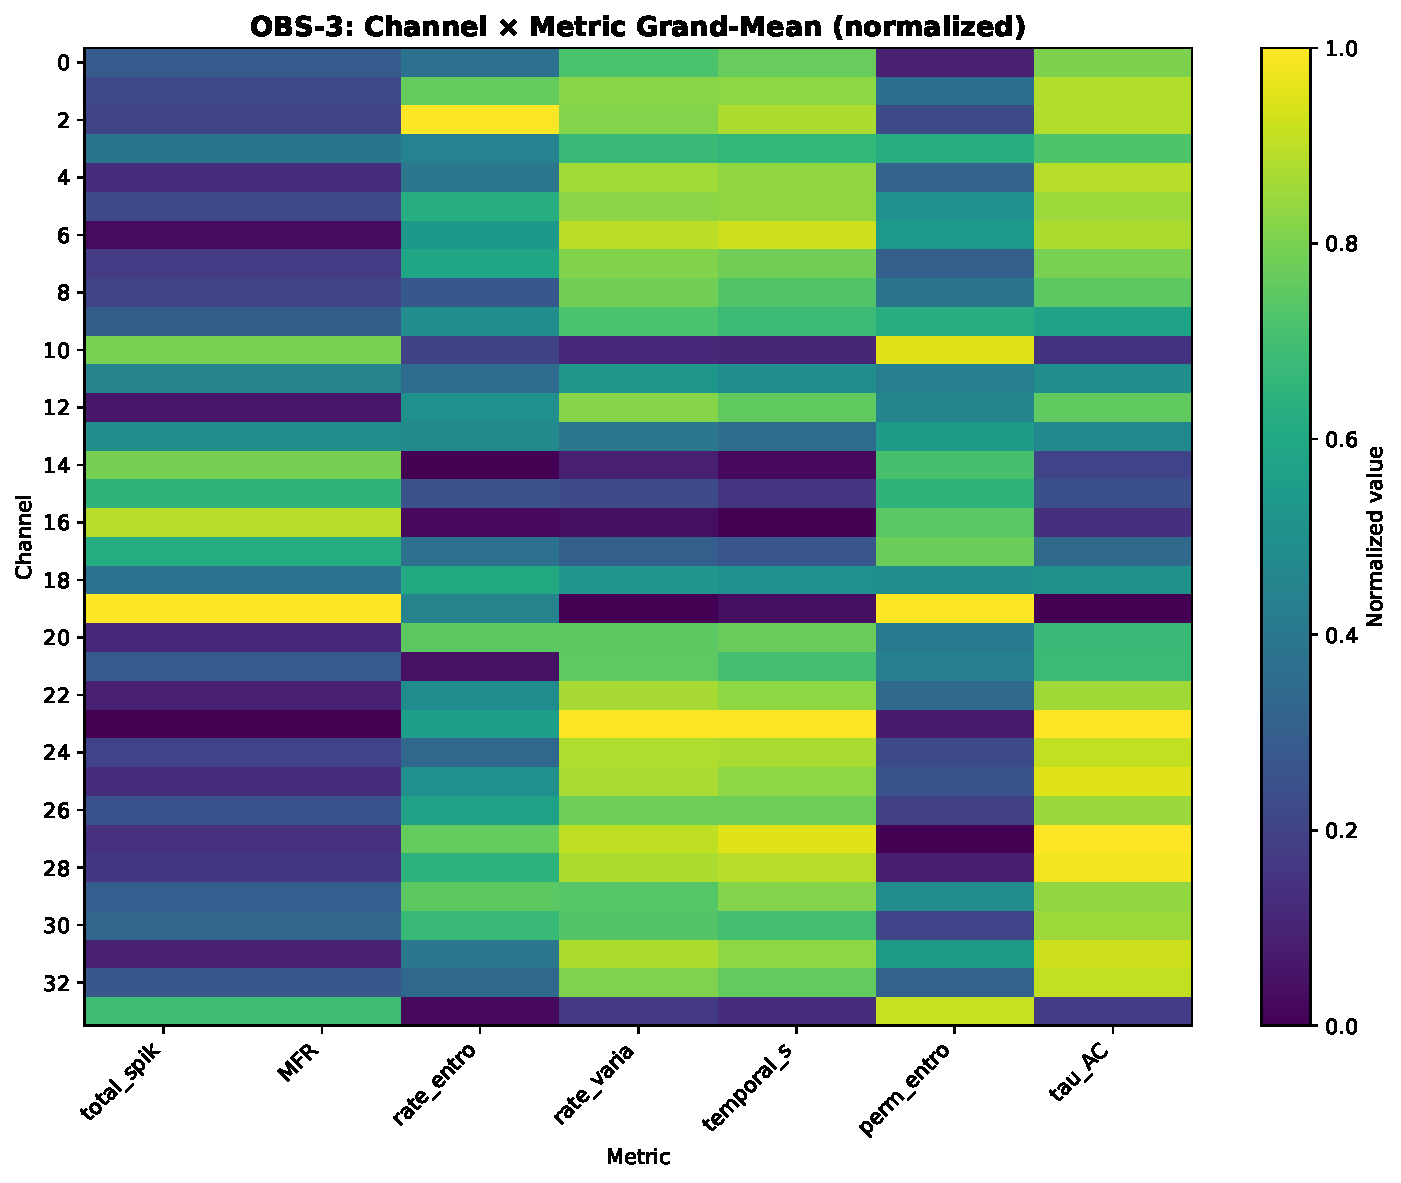
\includegraphics[width=\textwidth]{pictures/appendixA/obs03_channel_heterogeneity.pdf}
    \caption{OBS-3: Per-channel-index dynamical summaries. Temporal sparsity and $\tau_{\text{AC}}$ have maximum-to-minimum ratios of $2.54\times$ and $1.56\times$, respectively. Rate-entropy and permutation-entropy means vary less across the unlabeled channel indices.}
    \label{fig:app_ch6_obs03}
\end{figure}

\begin{figure}[H]
    \centering
    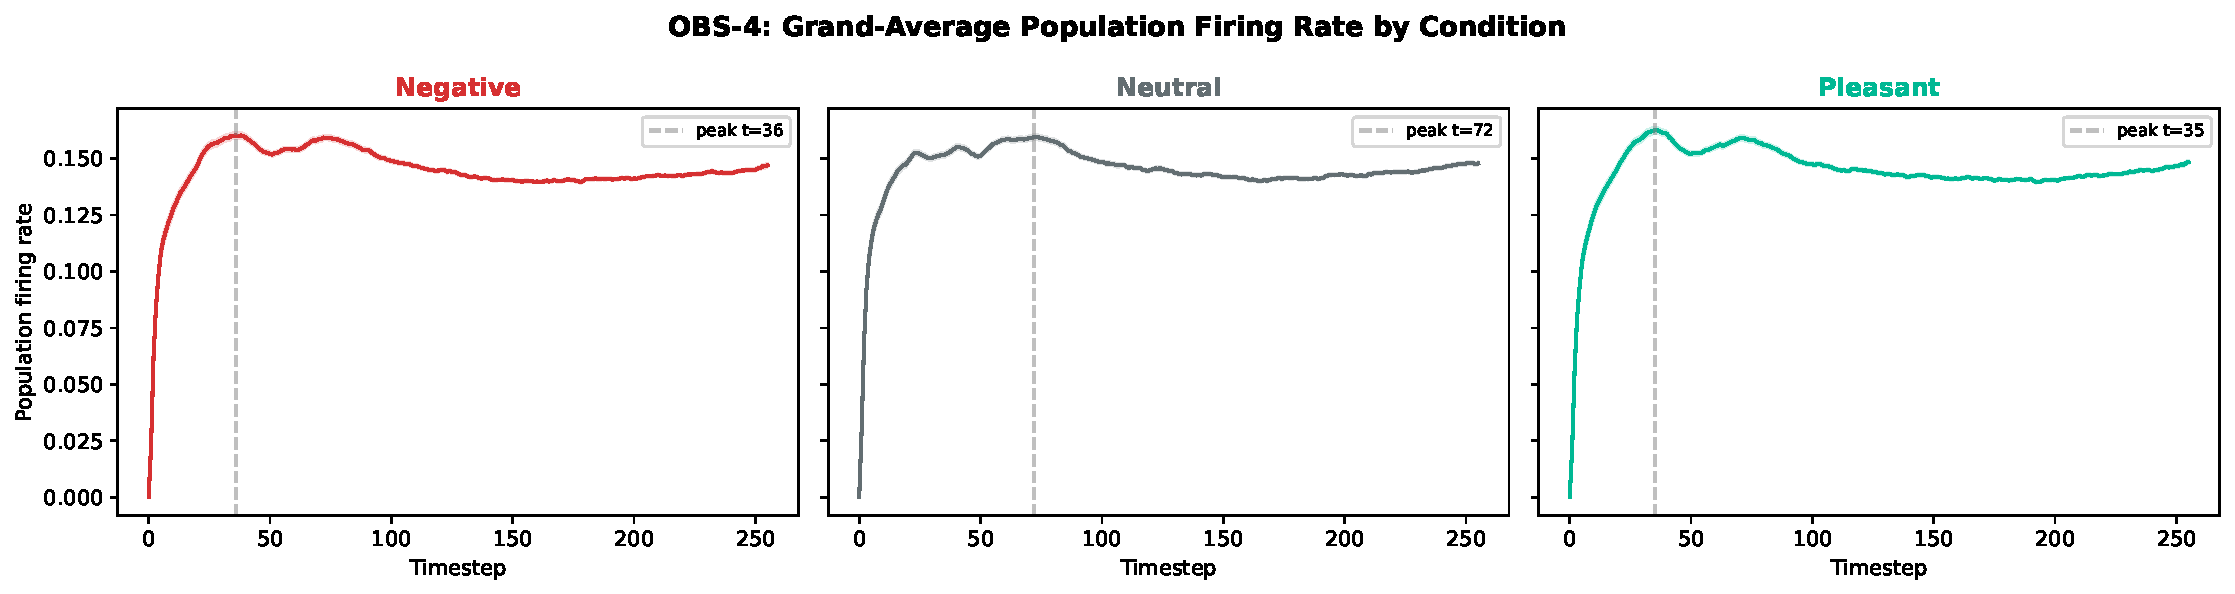
\includegraphics[width=\textwidth]{pictures/appendixA/obs04_firing_rate_timecourses.pdf}
    \caption{OBS-4: Grand-average reservoir population firing-rate traces. Negative and Pleasant peak at $t\approx35$--$36$, while Neutral peaks at $t=72$; the Pleasant peak-to-final ratio is $1.11$. These sample timings are descriptive and are not a validated measure of emotional salience.}
    \label{fig:app_ch6_obs04}
\end{figure}

\begin{figure}[H]
    \centering
    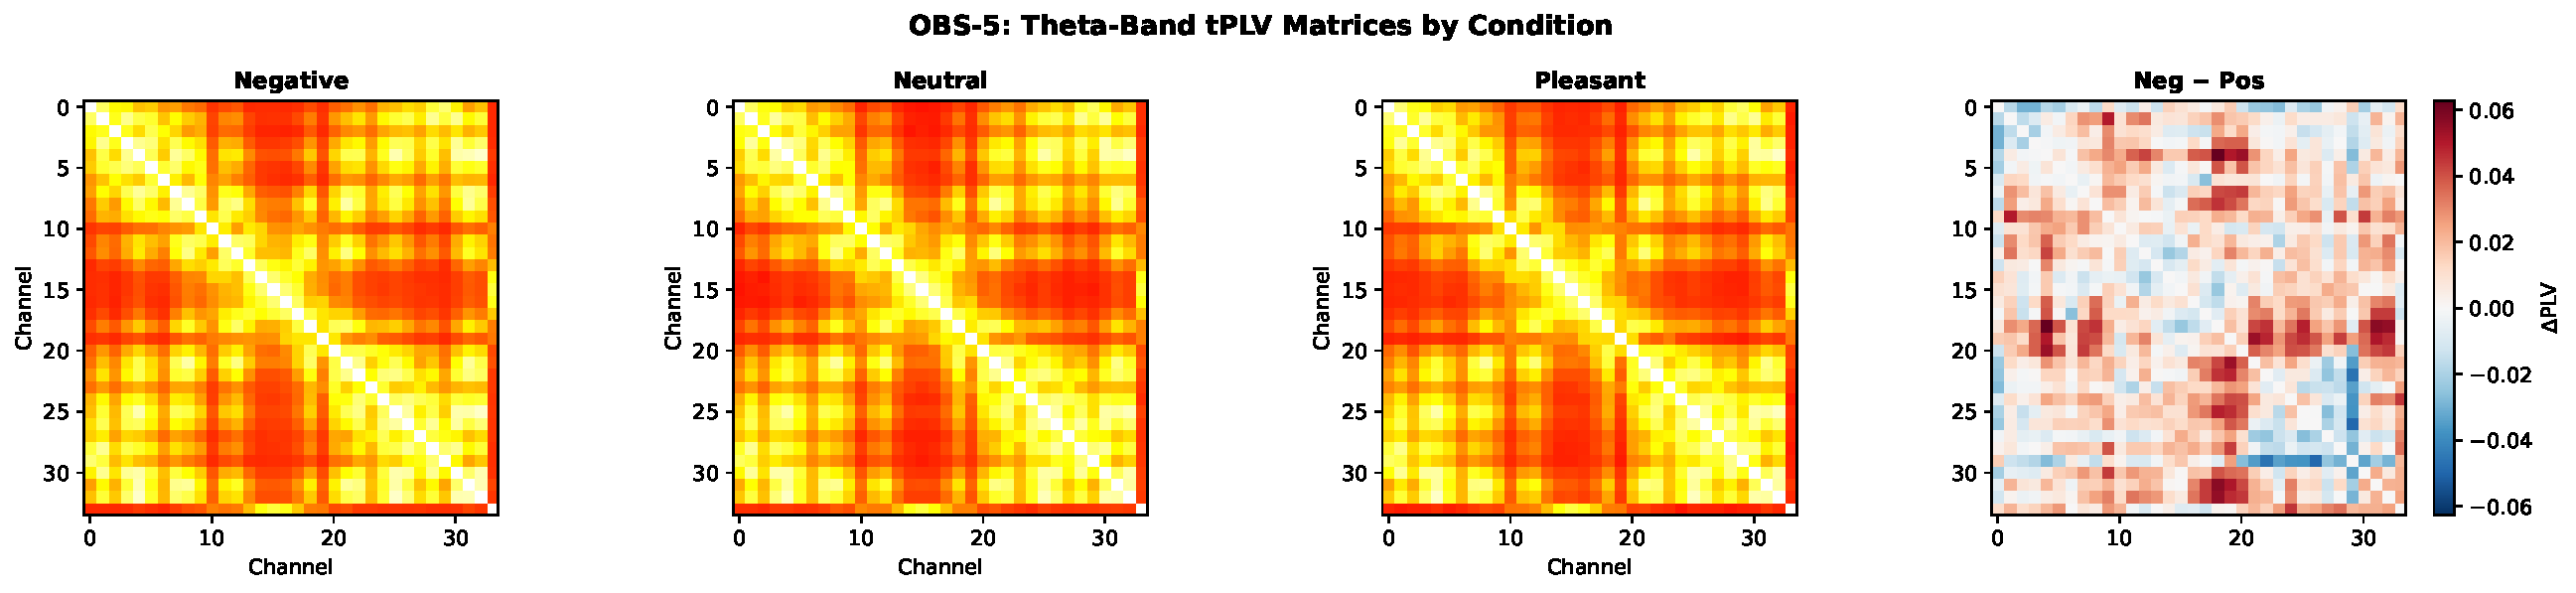
\includegraphics[width=\textwidth]{pictures/appendixA/obs05_tplv_connectivity.pdf}
    \caption{OBS-5: Archived theta-band within-epoch phase-concentration summaries. The displayed mean PLV values are Negative ($0.635$), Neutral ($0.632$), and Pleasant ($0.626$); the Negative--Pleasant mean $|\Delta\mathrm{PLV}|$ is $0.016$ (maximum $0.063$). With one trial-averaged epoch per participant--condition and unlabeled channels, these values are not interpreted as physiological connectivity.}
    \label{fig:app_ch6_obs05}
\end{figure}

\begin{figure}[H]
    \centering
    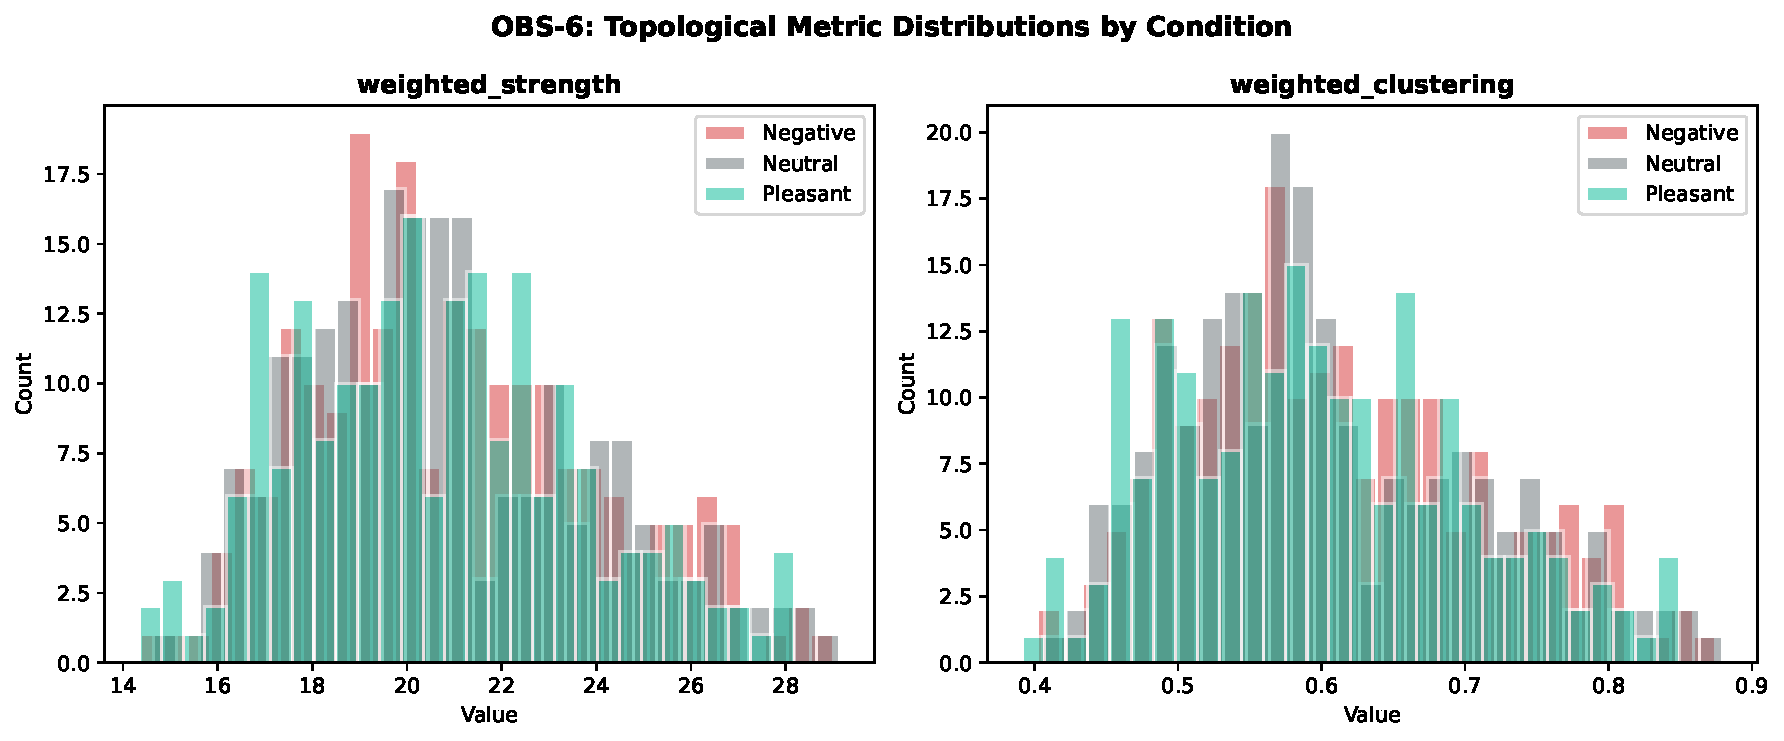
\includegraphics[width=\textwidth]{pictures/appendixA/obs06_topological_distributions.pdf}
    \caption{OBS-6: Archived graph-summary distributions. Weighted node strength ranges from $5.9$ to $30.8$, and weighted clustering from $0.21$ to $0.91$. The channel-index ranges permit the numerical association analysis in Chapter~\ref{chap:synthesis}, but they have no anatomical interpretation.}
    \label{fig:app_ch6_obs06}
\end{figure}

\begin{figure}[H]
    \centering
    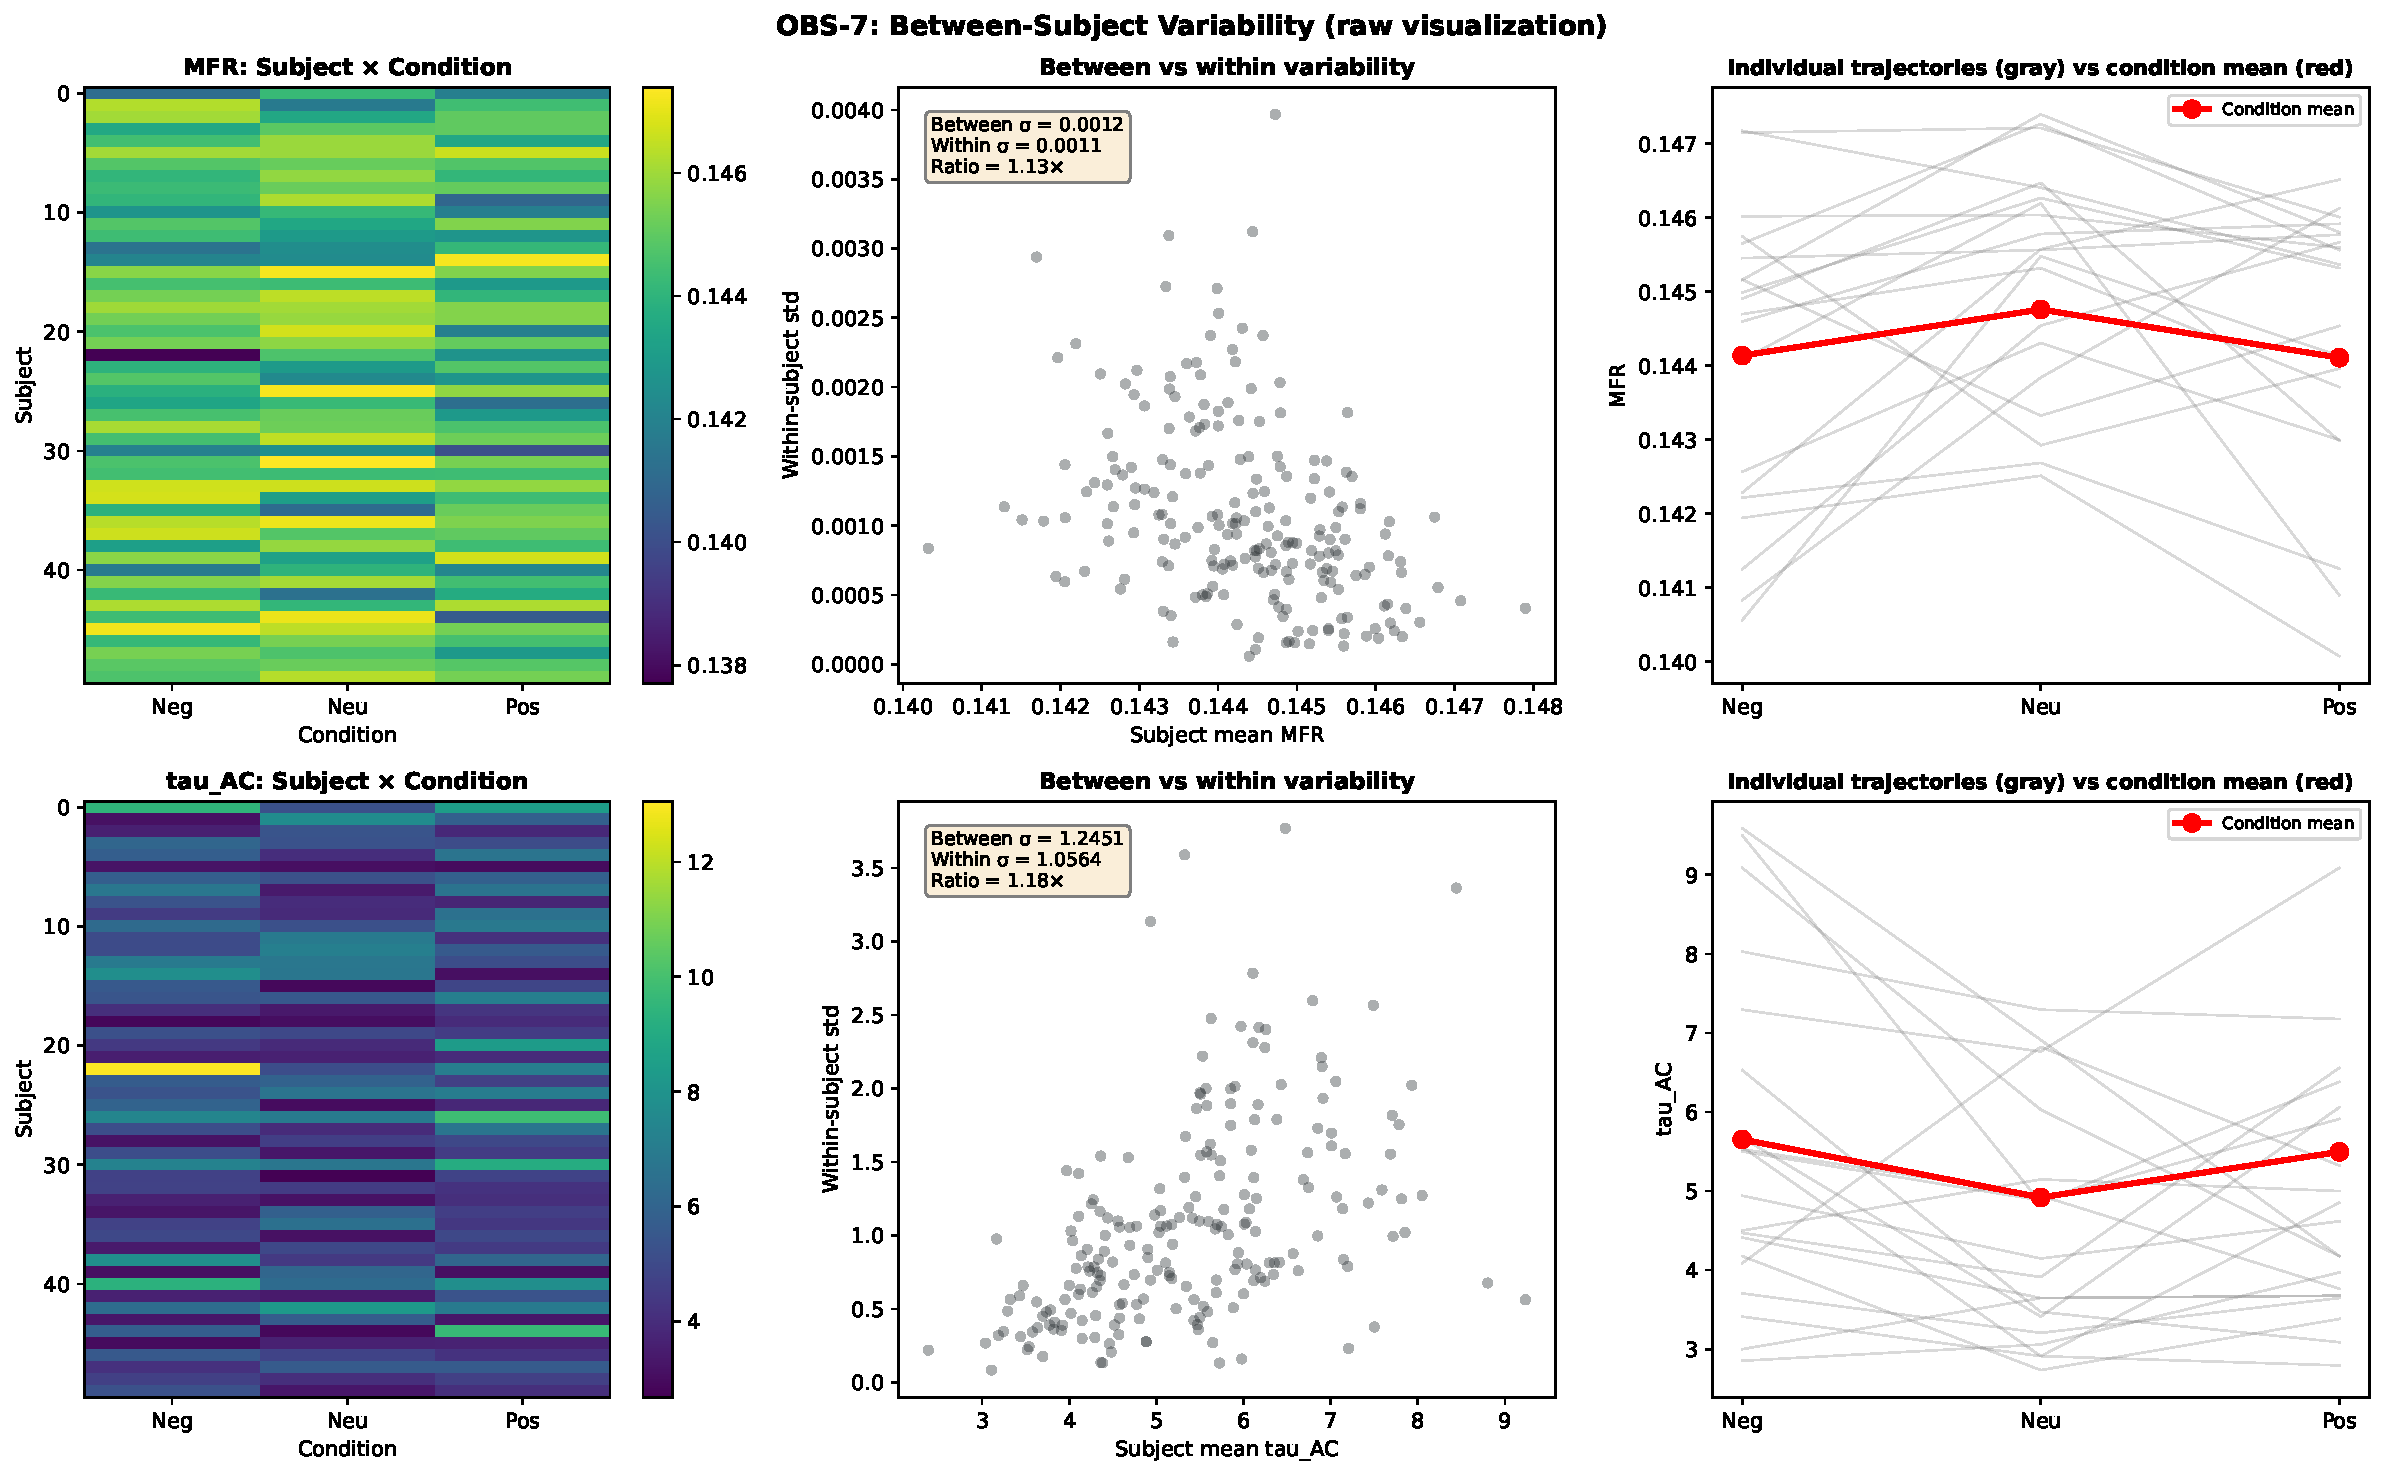
\includegraphics[width=\textwidth]{pictures/appendixA/obs07_subject_variability.pdf}
    \caption{OBS-7: Archived between-participant and within-participant variability summaries. The reported rate-entropy and permutation-entropy ratios are $0.87$ and $0.90$. These descriptive ratios are not test--retest reliabilities and are not directly comparable with the globally fitted BSC$_6$ PCA decomposition.}
    \label{fig:app_ch6_obs07}
\end{figure}

\begin{figure}[H]
    \centering
    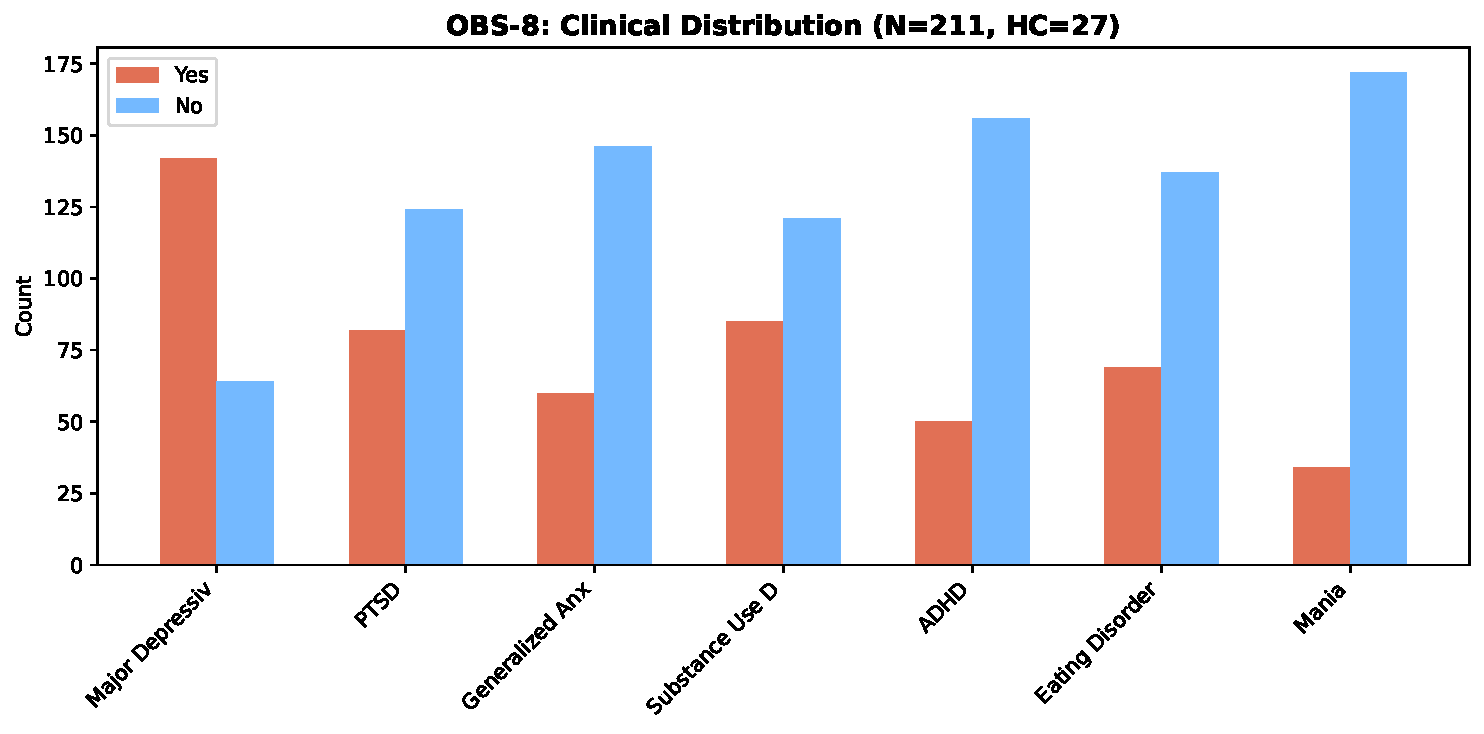
\includegraphics[width=\textwidth]{pictures/appendixA/obs08_clinical_distribution.pdf}
    \caption{OBS-8: Clinical metadata coverage. Complete five-diagnosis data are available for 206 of 211 subjects. MDD: 142 vs.\ 64; PTSD: 82 vs.\ 124; SUD: 85 vs.\ 121. Twenty-two complete cases are negative for all five primary diagnoses. The supplied full-panel comorbidity variable has mean 2.8 (rounded).}
    \label{fig:app_ch6_obs08}
\end{figure}



%% ═══════════════════════════════════════════════════════════════
%% SECTION A.5: CHAPTER 7
%% ═══════════════════════════════════════════════════════════════
\section{Chapter 7: Structure-Function Coupling}
\label{app:ch7_figs}

The five three-class coupling experiment figures (EXP-7.1 through EXP-7.5) are presented inline in Chapter~\ref{chap:synthesis}, Section~\ref{sec:ch7_3class}. The fourteen four-class coupling figures are presented inline in Sections~\ref{sec:exp7_coupling}--\ref{sec:exp7_augmentation} of the same chapter. No supplementary coupling figures are required.
